\documentclass{itkmitlcoop}

\usepackage{afterpage}
\usepackage{graphicx,amsmath,latexsym,amssymb,amsthm}
\usepackage{indentfirst}
\usepackage{cite}

\graphicspath{ {images/} }

\makeatletter
% \patchcmd{<cmd>}{<search>}{<replace>}{<succes>}{<failure>}
\patchcmd{\@chapter}{\addtocontents{lof}{\protect\addvspace{10\p@}}}{}{}{}% LoF
\patchcmd{\@chapter}{\addtocontents{lot}{\protect\addvspace{10\p@}}}{}{}{}% LoT
\makeatother

% Your thesis title (THAI)
\newcommand{\ThesisTiTle}{ชื่อโปรเจ็กต์จบ}
% Your thesis title (ENG)
\newcommand{\ThesisTiTleENG}{Project name}
% Your name
\newcommand{\AuName}{ชื่อ นามสกุล}
% Your name ENG
\newcommand{\AuNameENG}{Name Surname}
% Department / Program
\newcommand{\DepartmentENG}{Information Technology}
% Your student ID
\newcommand{\SId}{xx07xxxx}
% Your advisor
\newcommand{\Advisor}{ชื่อที่ปรึกษา}
% Your advisor
\newcommand{\AdvisorENG}{AdvisorName AdvisorSurname}
% Your advisor employee
\newcommand{\Exami}{ชื่อพนักงานที่ปรึกษา}
% ชื่อสถานประกอบการ
\newcommand{\Company}{ชื่อบริษัท}
% ภาคเรียนที่ (in normal letters)
\newcommand{\Sem}{1}
% ปีการศึกษา (in normal letters)
\newcommand{\AcaY}{2561}
% ปีการศึกษา (in normal letters)
\newcommand{\AcaYAD}{2018}
% วันส่งรายงาน
\newcommand{\SubD}{10 พฤศจิกายน พ.ศ. 2561}
% วันเริ่มทำงาน
\newcommand{\StartDWork}{23 กรกฎาคม พ.ศ. 2561}
% วันสุดท้ายของการทำงาน
\newcommand{\EndDWork}{30 พฤศจิกายน พ.ศ. 2561}
% ที่อยู่สถานประกอบการ
\newcommand{\Address}{ที่อยู่}
% เว็บไซต์สถานประกอบการ
\newcommand{\Website}{https://example.com}
% ตำแหน่งานที่ปฏิบัติ
\newcommand{\Position}{ตำแหน่งงานที่ปฏิบัติ}
%19. สาขาวิชา
\newcommand{\Department}{เทคโนโลยีสารสนเทศ}
\newcommand{\DepartmentENG}{Information Technology}

\begin{document}
    \frontmatter
    \pagenumbering{Roman}
    \lhead{}\rhead{}\chead{}\lfoot{}\cfoot{\thepage}\rfoot{}
    \makecover
    \makeinnercover
    \makeengcover
    \makecopyrightcover

    % Setting margin for page numbering on frontmatter
    \newgeometry{top=1in, bottom=1in, left=1.5in, right=1in, includefoot}

    \makeletter
    \makeack{
        \begin{enumerate}
            \item คุณ ชื่อ สกุล \quad ตำแหน่ง xxxxxxx (พนักงานที่ปรึกษา)
            \item คุณ ชื่อ สกุล \quad ตำแหน่ง xxxxxxx
        \end{enumerate}
    }
    \makeapproveletter
    \makeabstract{
    	บทคัดย่อ
    }

   \makeabstracteng{
       Abstract
   }

    \newpage
    \addcontentsline{toc}{chapter}{สารบัญ}
    \tableofcontents

    \newpage
    \addcontentsline{toc}{chapter}{สารบัญตาราง}
    \listoftables

    \newpage
    \addcontentsline{toc}{chapter}{สารบัญภาพ}
    \listoffigures

    % Reset frontmatter page numbering margin, back to original margin from class file
    \restoregeometry

    \mainmatter
    \lhead{}\rhead{\thepage}\chead{}\lfoot{}\cfoot{}\rfoot{}

    \chapter{บทนำ}
\label{chapter:introduction}

\section{ที่มาและความสำคัญ}

การ์ตูนญี่ปุ่นเป็นที่รู้จักกันอย่างแพร่หลายทั่วโลกในฐานะสื่อบันเทิง หรืออีกชื่อหนึ่งคือ “มังงะ (Manga)” ในปัจจุบันมีงานวิจัยในหัวข้อมังงะอย่างหลากหลาย ในหลาย ๆ งานวิจัย~\cite{8369633, Liu2016, Pang2014, 7415523, ogawa2018, 7351614, 7452668} มีการใช้ชุดข้อมูลสำหรับการทดลอง เช่น Manga109~\cite{Matsui2017} ซึ่งเป็นชุดข้อมูลที่ถูกสร้างขึ้นจากภาพมังงะจำนวน 20,260 หน้า รวบรวมจากมังงะ 109 เรื่อง มังงะที่ถูกรวบรวมมานี้เป็นผลงานของนักวาดมังงะมืออาชีพชาวญี่ปุ่น นอกจากภาพของมังงะแล้ว ชุดข้อมูลนี้ยังประกอบไปด้วยข้อมูลอธิบายประกอบ หรือ Annotation ต่าง ๆ เช่น ขอบเขตและตำแหน่งของใบหน้า ร่ายกาย และ กรอบภาพ เป็นต้น นอกจากนี้ยังมีข้อมูลขอบเขตและตำแหน่งของข้อความที่ปรากฎในภาพมังงะ โดยตำแหน่งข้อความต่าง ๆ นั้นถูกป้อนข้อมูลด้วยแรงงานคนโดยไม่พึ่งพาระบบอัตโนมัติใด ๆ ในการป้อนข้อมูลดังกล่าวนั้นใช้เวลานานและต้องพึ่งพาแรงงานมนุษย์ ด้วยเหตุนี้ระบบอัตโนมัติที่จะสามารถเข้ามาช่วยในการระบุข้อมูล Annotation นั้นจึงมีประโยชน์และสามารถช่วยลดภาระงานในส่วนนี้ลงได้อย่างมาก

ถึงแม้ว่าสำหรับภาพวาดรูปแบบการ์ตูนญี่ปุ่นจะมีทั้งแบบภาพวาดทั่วไปที่เป็นภาพแสดงของตัวละครหรือทิวทัศน์และแบบภาพมังงะ แต่ภายในงานวิจัยนี้เรามุ่งเน้นไปที่มังงะเป็นหลักเนื่องจากข้อความมักปรากฎบนหนังสือการ์ตูนมากกว่าภาพวาดทั่วไปอย่างที่ทราบกันดี สำหรับวิธีการตรวจหาข้อความในภาพมังงะนั้นมีการพัฒนามาหลากหลายก่อนหน้านี้~\cite{6761596, 7490104} แต่วิธีเหล่านี้ถูกพัฒนาให้พึ่งพาโครงสร้างส่วนต่าง ๆ ของภาพมังงะเป็นข้อมูลอ้างอิง เช่น กรอบช่องภาพวาด, ลักษณะของกล่องคำพูด เป็นต้น นอกจากนี้บางวิธียังคงมีความจำเป็นที่ต้องพึ่งพาการป้อนข้อมูลเข้าจากภายนอกทั้งจากมนุษย์และข้อมูลอื่น ๆ ทำให้ไม่สามารถทำงานได้อัตโนมัติอย่างสมบูรณ์ อย่างไรก็ดีไม่นานมานี้มีการพัฒนาวิธีการใหม่โดยใช้วิธีการ Deep Learning อย่างเช่นเทคนิค Convolutional Neural Network เพื่อช่วยในการสกัดลักษณะเด่น (Feature) ออกจากภาพมังงะเพื่อช่วยในการตรวจหาข้อความในภาพมังงะ~\cite{7532890} ซึ่งวิธีการนี้สามารถเพิ่มความแม่นยำและถูกต้องในการตรวจหาข้อความได้โดยปราศจากการพึ่งพาโครงสร้างต่าง ๆ ในภาพมังงะ แต่อย่างไรก็ดี Deep Learning ยังเป็นการวิธีการที่ต้องใช้ทรัพยากรของระบบเพื่อการคำนวนมากกว่าวิธีการอื่น ๆ ซึ่งเป็นข้อเสียสำคัญประการหนึ่ง~\cite{7532890}

ในงานวิจัยนี้มีจุดมุ่งหมายเพื่อพัฒนาระบบตรวจหาข้อความที่ทำงานได้กับมังงะอย่างหลากหลายและไม่ถูกจำกัดด้วยโครงสร้างหรือลักษณะบางประการของภาพมังงะ เราจึงเลือกใช้ Stroke Width Transform (SWT) ในการสกัดลักษณะเด่นของเส้นต่าง ๆ ของวัตถุที่ปรากฎในภาพออกมา โดยวิธีการนี้ถูกใช้เป็นขั้นตอนแรกของการตรวจหาข้อความบนภาพถ่ายมาก่อนหน้านี้ วิธีการนี้ทำงานโดยพึ่งพาสมมติฐานว่าขอบของเส้นอักษรในข้อความนั้นมีขอบที่ชัดเจนและหนาแน่นปรากฏอยู่บนพื้นหลังที่ราบเรียบ~\cite{5540041} อย่างไรก็ดีการใช้วิธีการนี้กับการตรวจหาข้อความบนภาพมังงะส่งผลให้เกิดข้อผิดพลาดเชิง False Positive จำนวนมาก ปัญหานี้เกิดจากความแตกต่างของลักษณะเฉพาะตัวของภาพถ่ายและภาพวาดมังงะ ภาพมังงะนั้นโดยส่วนใหญ่มีลักษณะเป็นภาพขาวดำ และลักษณะของวัตถุภายในมังงะ เช่น ขนาด, เส้น, และพื้นหลัง นั้นมีความคล้ายคลึงกับตัวอักษรของข้อความ ด้วยปัญหาข้างต้นเราจึงตั้งเป้าหมายในการปรับปรุงและพัฒนา SWT ที่ถูกใช้ในภาพถ่าย~\cite{5540041} เพื่อให้สามารถทำงานกับภาพมังงะได้

วิธีการใหม่ของเราที่ถูกพัฒนาขึ้นใหม่นั้นแบ่งออกเป็น 4 ส่วนดังนี้ (\rNum{1}) The Stroke Width Transform (\rNum{2}) ค้นหาวัตถุที่เข้าข่ายลักษณะของตัวอักษร (\rNum{3}) คัดแยกอักษร โดยใช้ Support Vector Machine (SVM) ร่วมกับ Histogram of Oriented Gradients Feature (\rNum{4}) จัดกลุ่มอักษรที่ผ่านการคัดแยกแล้วให้เกิดเป็นบรรทัดหรือกลุ่มของข้อความ

\section{วัตถุประสงค์}
พัฒนาระบบค้นหาตำแหน่งข้อความสำหรับมังงะ โดยนำ Stroke Width Transform ที่ถูกใช้เป็นกระบวนการแรกเริ่มในเทคนิคตรวจหาข้อความบนภาพถ่ายมาพัฒนาและปรับปรุงต่อยอดเพื่อให้สามารถใช้งานกับภาพมังงะได้มีประสิทธิภาพมากขึ้น

\section{ขอบเขตของงานวิจัย}
\begin{enumerate}
    \item พัฒนาระบบตรวจหาตำแหน่งข้อความซึ่งใช้สำหรับภาพมังงะ โทนสีขาวดำ
    \item ภาษาของเนื้อหาในมังงะที่นำมาใช้งาน คือ ภาษาญี่ปุ่น
    \item ข้อมูลที่ใช้ในการวิจัยเพื่อการเทรนและทดสอบนำมาจากฐานข้อมูล Manga109
\end{enumerate}

\section{ประโยชน์ที่คาดว่าจะได้รับ}
\begin{enumerate}
    \item ได้วิธีการตรวจหาข้อความใหม่ที่ถูกพัฒนาขึ้นเพื่อใช้งานร่วมกับภาพมังงะโดยเฉพาะ
    \item ทำให้ทราบถึงลักษณะที่เป็นเอกลักษณ์ของมังงะซึ่งแตกต่างจากภาพถ่ายทั่วไป
\end{enumerate}



    \chapter{การทบทวนวรรณกรรมที่เกี่ยวข้อง}
\label{chapter:literature-review}

ในบทที่ 2 จะอธิบายถึงทฤษฎีที่เกี่ยวข้องในการสร้างแบบจำลองการระบุสายพันธุ์นก
ซึ่งประกอบด้วย ทฤษฎีเสียงและสัญญาณ (Sound and Signal) 
ทฤษฎีการประมวลผลภาพดิจิตัล (Digital Image Processing) ทฤษฎีการเรียนรู้ของเครื่อง (Machine Learning)
โครงข่ายประสาทเทียม (Artificial Neural Network) โครงข่ายประสาทเชิงลึก (Deep Neural Network) 
โครงข่ายประสาทแบบคอนโวลูชัน (Convolutional Neural Network, CNN) สถาปัตยกรรมต่าง ๆ ของโครงข่ายประสาทแบบคอนโวลูชันและการกำหนดองค์ประกอบ (CNN Architecture and Configuration)
เมตริกที่ใช้ในประเมินผลแบบจำลอง (Evaluation Metrics) และหลักการทำงานของเครื่องมือต่าง ๆ ที่ใช้ในงานวิจัย

\section{เสียงและสัญญาณ (Sound and Signal)}
เสียงเป็นพลังงานรูปแบบหนึ่งที่เกิดจากการสั่นสะเทือนของแหล่งกำเนิดเสียงผ่านตัวกลางและรับรู้ได้ด้วยหู ส่วนสัญญาณเป็นการแสดงถึงปริมาณที่แปรผันตามเวลา
ซึ่งมีคำจำกัดความที่ค่อนข้างเป็นนามธรรม และสัญญาณเสียงจะแสดงถึงความแปรปรวนของความกดอากาศเมื่อเวลาผ่านไป 
โดยมีไมโครโฟนที่ทำหน้าที่ในการวัดความแปรผันและสร้างสัญญาณไฟฟ้าที่เป็นตัวแทนของเสียง
และมีลำโพงที่ทำหน้าที่ในการรับสัญญาณไฟฟ้าและทำให้เกิดเสียง ซึ่งทั้งไมโครโฟนและลำโพงจะถูกเรียกว่า 
ทรานดิวเซอร์ (transducer) เนื่องจากทั้งไมโครโฟนและลำโพงเป็นอุปกรณ์ที่ทำหน้าที่รับพลังงานจากรูปแบบหนึ่ง
แล้วแปลงไปให้อยู่ในอีกรูปแบบหนึ่ง

\subsection{สัญญาณซ้ำคาบ (Periodic signals)}
เป็นลักษณะของสัญญาณที่มีรูปแบบการเกิดที่ซ้ำกันในหนึ่งช่วงเวลาที่เท่า ๆ กัน เรียกการวนครบรูปแบบของสัญญาณหนึ่งครั้งว่ารอบ (cycle) 
และเรียกระยะเวลาในแต่ละรอบว่าคาบ (period)  สัญญาณนี้จะมีลักษณะคล้ายกับกราฟของฟังก์ชันไซน์ ดังภาพ~\ref{Fig:Sine_wave}

\begin{figure}[h]
    \centering
    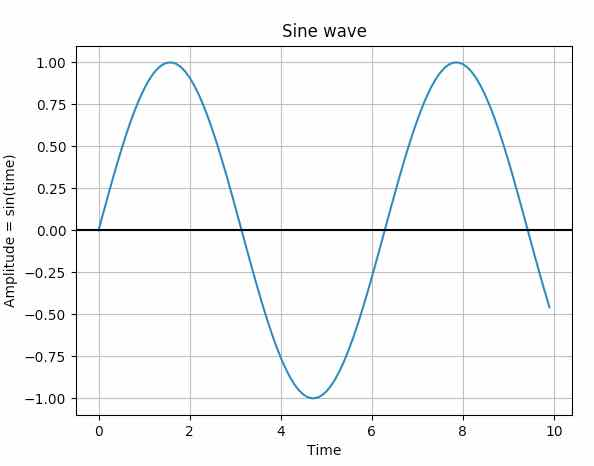
\includegraphics[scale = 0.3]{sinewave.jpg}
    \caption{แสดงกราฟของฟังก์ชันไซน์}
    \label{Fig:Sine_wave}
\end{figure}

ความถี่ของสัญญาณมีหน่วยเป็นจำนวนของรอบต่อวินาที ซึ่งเป็นค่าที่ตรงกันข้ามกับคาบ ซึ่งมีหน่วยคือ รอบต่อวินาที หรือ เฮิรตซ์ (Hz) 
ในเครื่องดนตรีส่วนใหญ่จะให้สัญญาณซ้ำคาบเพียงแต่ไม่ได้อยู่ในรูปแบบของสัญญาณไซน์ (sinusoidal) 
ตัวอย่างเช่นสัญญาณของเสียงไวโอลิน

\begin{figure}[h]
    \centering
    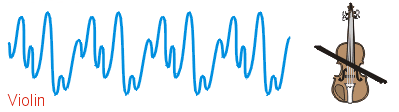
\includegraphics[scale = 0.5]{violin_waveform.png}
    \caption{แสดงสัญญาณซ้ำคาบ}
    \label{Fig:Periodic_signal}
\end{figure}
% \begin{figure}[h]
%     \includegraphics[]{}
%     \caption{}
%     \label{}
% \end{figure}

เราเรียกรูปร่างของสัญญาณซ้ำคาบเหล่านี้ว่า รูปแบบของคลื่น (waveform) เครื่องดนตรีส่วนใหญ่จะสร้างรูปแบบของคลื่นที่ซับซ้อนมากกว่าสัญญาณไซน์ 
รูปแบบของคลื่นจะเป็นเครื่องกำหนดลักษณะของเสียงร้องหรือเสียงดนตรี ดังภาพ~\ref{Fig:Periodic_signal} ซึ่งเป็นการรับรู้เกี่ยวกับคุณภาพของเสียง 
และมนุษย์มักจะรับรู้เสียงที่มีความซับซ้อนมากกว่ารูปแบบคลื่นของไซน์ 

\subsection{สัญญาไม่ซ้ำคาบ (Non-periodic signals)}
เป็นสัญญานที่มีการเปลี่ยนแปลงที่ไม่สามารถระบุรูปแบบที่แน่นอนของสัญญาณได้ เช่นเสียงการพูดคุยของมนุษย์ 
สัญญาณเหล่านี้สามารถมองเห็นได้โดยการนำเสนอในรูปแบบของเสปกโตรแกรม (spectrograms)

\subsection{การสุ่มตัวอย่าง (Sampling)}
การสุ่มตัวอย่างคือการเปลี่ยนแปลงสัญญาณที่มีความต่อเนื่องทางเวลา (Continuos signal) ให้อยู่ในรูปแบบที่ไม่ต่อเนื่องทางเวลา (Discrete signal) ด้วยการสุ่มเก็บตัวอย่างของสัญญาณ
ในช่วงเวลาที่ห่างเท่า ๆ กัน ซึ่งช่วงเวลาดังกล่าวจะถูกเรียกว่า อัตราสุ่มสัญญาณ (Sampling rate) ในการสุ่มสัญญาณจำเป็นต้องเลือกอัตราการสุ่มให้เหมาะสมกับความถี่ของสัญญาณนั้น ๆ
เนื่องจากในเวลาที่ต้องการแปลงสัญญาณกลับไปเป็นสัญญาณที่มีความต่อเนื่องทางเวลาจะได้สัญญาณต้นฉบับที่ถูกต้องและครบถ้วน~\cite{AT1987}

\subsection{สเปกโตรแกรม (Spectrograms)}
สเปกโตรแกรมเป็นภาพหรือแผนภาพของสเปกตรัม(Spectrum) โดยที่สเปกตรัมเป็นแถบคลื่นความถี่ของเสียงที่รวมกับแสงที่มนุษย์สามารถมองเห็นได้ 
โดยสเปกโตรแกรมทำให้สามารถมองเห็นผลลัพธ์ของการแบ่งเสียงออกเป็นส่วน ๆ ได้ โดยเรียกการเปลี่ยนของเสียงในแต่ละส่วนละส่วนเป็นสเปกโตรแกรมนี้จะถูกเรียกว่า Short-Time Fourier Transform (STFT)
โดยที่แกน x ของสเปกโตรแกรมจะแสดงเวลาและแสดงความถีบนแกน y โดยในแต่ละคอลัมน์จะแสดงสเปกตรัมของส่วนนั้น ๆ โดยใช้สีในการแสดงแอมพลิจูด (Amplitude) หรือความเข้มของเสียงนั้น

\begin{figure}[h]
    \centering
    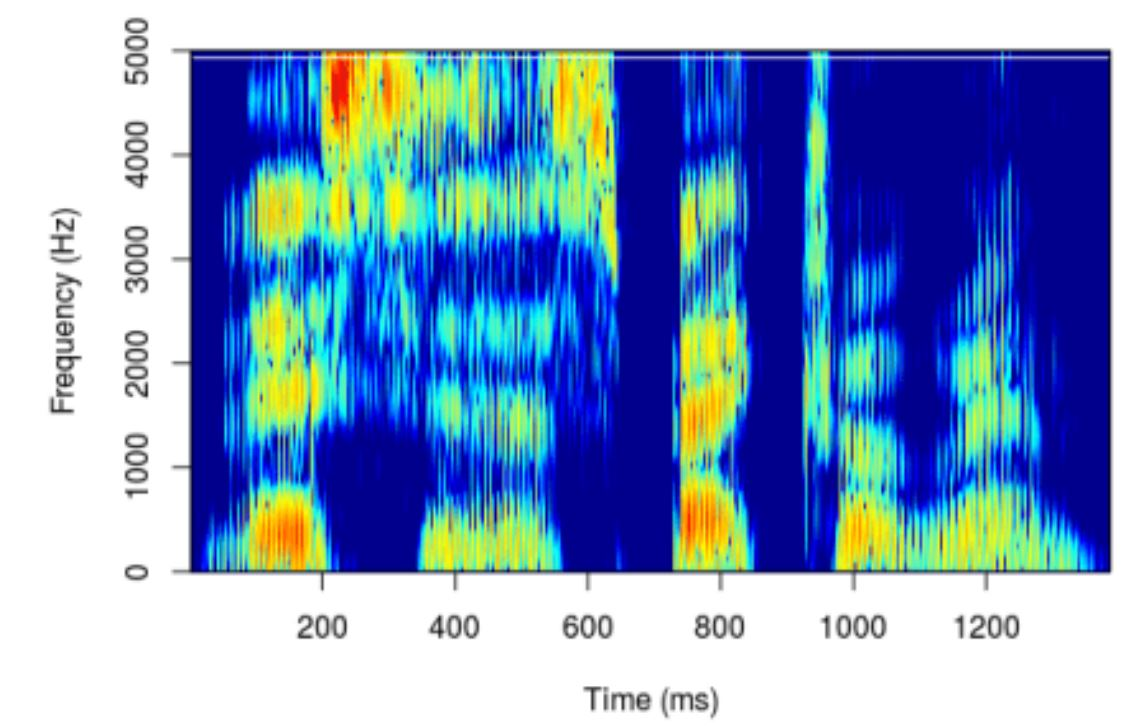
\includegraphics[scale = 0.4]{spectogram_1.JPG}
    \caption{แสดงตัวอย่างภาพสเปกโตรแกรม}
    \label{Fig:specto_gram_1}
\end{figure}

\subsection{สัญญาณรบกวน (Noise)}
เป็นเสียงหรือสัญญาณที่ไม่พึงประสงค์ที่อาจเกิดจากการทำงานผิดพลาดของอุปกรณ์ที่ใช้ในการเก็บข้อมูล หรือสร้างขึ้นเพื่อศึกษาลักษณะ รูปแบบ และทำความเข้าใจกับสัญญาณรบกวนเหล่านี้ได้
โดยสัญญาณรบกวนที่สร้างง่ายที่สุดถูกเรียกว่า เสียงสัญญาณรบกวนที่ไม่เกี่ยวข้องกันแบบสม่ำเสมอ (Uncorrelated Uniform Noise) หรือ UU Noise โดยที่ Uniform หมายถึงสัญญาณจะมีการสุ่มค่าจากการกระจายที่สม่ำเสมอ 
นั่นคือทุก ๆ ค่าในช่วงนั้นมีโอกาสที่จะเท่ากัน และ uncorrelated ที่หมายถึงไม่เกี่ยวข้องกันหรือเป็นอิสระต่อกัน กล่าวคือการรู้ค่าเพียงค่าเดียวไม่สามารถให้ข้อมูลอื่น ๆ ได้
และมี 3 สิ่งที่ควรทราบเกี่ยวกับสัญญาณรบกวนและสเปกตรัมคือ 1. การกระจายของสัญญาณสุ่ม 2. ความสัมพันธ์ของแต่ละค่าในสัญญาณเป็นอิสระจากกันหรือไม่ 
และ 3. ความสัมพันธ์ระหว่างกำลัง (Power) กับความถี่ จากสามสิ่งที่ควรทราบนี้จะสามารถสร้างสัญญาณรบกวนได้ 3 ลักษณะคือ สัญญาณรบกวนบราวน์ (Brownian noise) 
หรือสัญญาณรบกวนสีแดง (Red noise) สัญญาณรบกวนสีชมพู (Pink Noise) และ Gaussian Noise หรือสัญญาณรบกวนสีขาว สัญญาณรบกวนโดยปกติจะถูกสังเคราะห์ขึ้นจากสมการ~\ref{eq:noise_generate}

\begin{equation}
    P = \frac{K}{f^{\beta}}
    \label{eq:noise_generate}
\end{equation}

โดยที่ $P$ คือกำลัง $f$ เป็นค่าของความถี่และ $K$ คือจุดตัดของเส้นตรง จากสมการข้างต้นเราสามารถทราบความสัมพันธ์ระหว่างกำลังและความถี่ของสัญญาณรบกวนต่าง ๆ ได้ คือเมื่อ
$P = K / f^{2}$ ผลลัพธ์ของสัญญาณรบกวนนี้จะตกอยู่ในช่วงของสเปกตรัมแสงสีแดง ซึ่งมีความถี่ที่ต่ำที่สุด ในขณะที่ถ้าเราเปลี่ยนค่าของ $\beta$ ให้เท่ากับ 0 สัญญาณรบกวนที่เกิดขึ้นจะตกอยู่ในช่วงของสเปกตรัมแสงสีขาว 
ทำให้เกิดเป็นสัญญาณรบกวนสีขาว และเมื่อค่า $\beta$ มีค่าอยู่ในระหว่าง 0 ถึง 2 ผลลัพธ์ของสัญญาณรบกวนจะอยู่ระหว่างช่วงสเปกตรัมแสงสีขาวและสีแดง จึงเรียกสัญญาณรบกวณที่อยู่ในช่วงนี้ว่าสัญญาณณบกวนสีชมพู

\section{ทฤษฎีการประมวลผลภาพดิจิตัล (Digital Image Processing)}

\section{การเรียนรู้ของเครื่อง (Machine Learning)}
การเรียนรู้ของเครื่องคือการที่คอมพิวเตอร์สามารถที่จะเรียนรู้ได้ด้วยตัวเอง โดยที่ไม่ต้องเขียนโปรแกรมสั่งให้คอมพิวเตอร์ทำงาน 
ซึ่งจะแตกต่างกับการเขียนโปรแกรมในสมัยก่อน ซึ่งในสมัยก่อนโปรแกรมเมอร์ต้องทำการโปรแกรมไปยังคอมพิวเตอร์เพือให้ได้ผลลัพธ์ออกมา 
แต่ในการเรียนรู้ของเครื่องผู้ใช้งานเพียงแค่ใส่ข้อมูลและระบุผลลัพธ์ที่ต้องการเท่านั้น 
คอมพิวเตอร์จะทำการเรียนรู้ด้วยตนเองแล้วแสดงผลลัพธ์ที่ได้ออกมาเป็นโปรแกรมที่สามารถนำไปใช้ในการทำนายผลลัพธ์ของข้อมูลได้ดังรูป~\ref{Fig:tradition_vs_ml}

\begin{figure}[h]
    \centering
    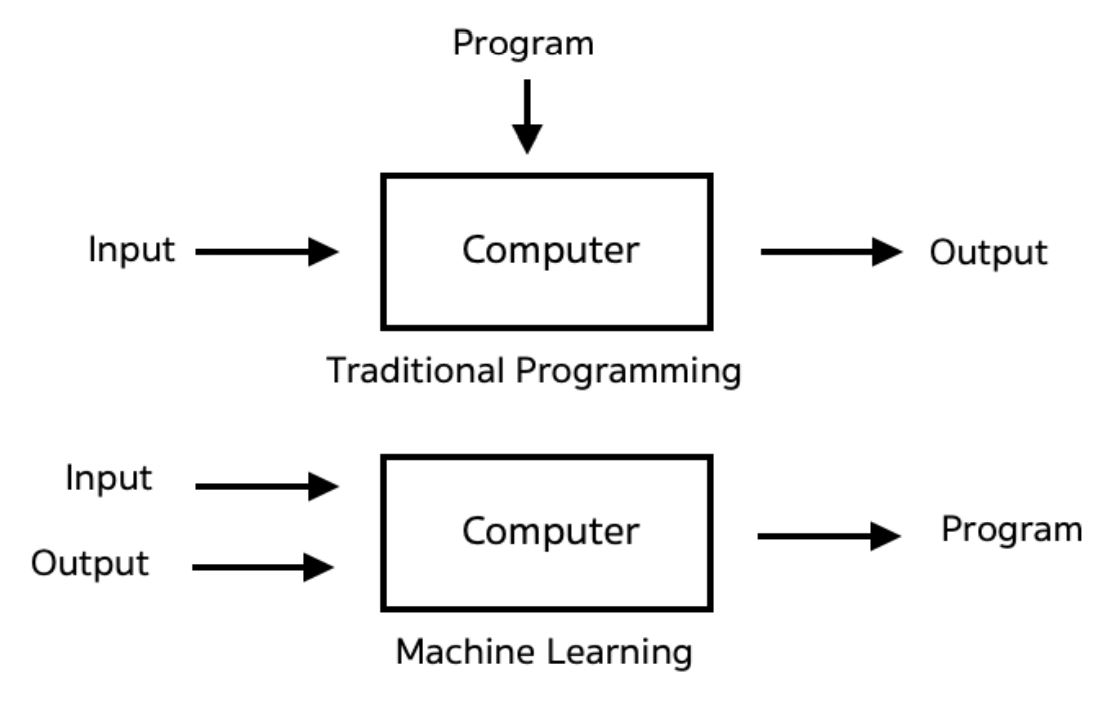
\includegraphics[scale = 0.4]{tradition_v_ml.JPG}
    \caption{แสดงความแตกต่างระหว่างการเขียนโปรแกรมในอดีตกับการเรียนรู้ของเครื่อง}
    \label{Fig:tradition_vs_ml}
\end{figure}
\FloatBarrier

โดยการเรียนรู้ของเครื่องนั้นจะประกอบไปด้วยข้อมูลและเครื่องมือทางสถิติที่ใช้ในการทำนายผลลัพธ์หรือหารูปแบบของข้อมูลที่เข้าไป
เครื่องจะทำการเรียนรู้ที่มีลักษณะคล้ายกันกับมนุษย์คือเรียนรู้จากประสบการณ์ 
ยิ่งมีประสบการณ์มากก็จะยิ่งมีความเชี่ยวชาญมากทำให้ง่ายต่อการทำนายผลลัพธ์ที่เกิดขึ้นจากสถานการณ์ที่คล้าย ๆ กันได้
และเพื่อเพิ่มความแม่นยำในการทำนายผลลัพธ์ เครื่อง (Machine) ก็ควรจะมีการฝึกด้วยข้อมูลจำนวนที่มากเพียงพอ 
ที่เครื่องจะสามารถค้นพบผลลัพธ์ผ่านรูปแบบหรือแบบแผนที่ซ้ำ ๆ กันได้ และการเรียนรู้ของเครื่องนั้นสามารถแบ่งรูปแบบการเรียนรู้ได้เป็น 2 ลักษณะใหญ่ ๆ คือ

\subsection{การเรียนรู้แบบมีผู้สอน (Supervised Learning)}
การเรียนรู้แบบมีผู้สอนคือการที่คอมพิวเตอร์สามารถหาผลลัพธ์ของข้อมูลได้ดัวยตัวเองหลังจากที่มีการเรียนรู้จากชุดข้อมูลตัวอย่างไปแล้วระยะเวลาหนึ่ง 
โดยเริ่มต้นโปรแกรมเมอร์จะเขียนโปรแกรมให้คอมพิวเตอร์สร้างแบบจำลอง (Model) 
ขึ้นมาจากชุดข้อมูลและผลลัพธ์ตัวอย่าง โดยที่ถ้าชุดข้อมูลตัวอย่างมีความหลากหลายและมีจำนวนมากอาจทำให้ผลลัพธ์ที่ได้จากการเรียนรู้นั้นมีความแม่นยำมากขึ้น 
กระบวนการนี้จะถูกเรียกว่าการฝึกอบรม(Train) เมื่อผลลัพธ์ที่ได้มีความแม่นยำมากขึ้น 
จะกล่าวได้ว่าแบบจำลองที่ได้จากการฝึกอบรมนี้มีความสามารถในการทำนายผลลัพธ์ได้ถูกต้องมากขึ้น 
การเรียนรู้แบบมีผู้สอนสามารถแบ่งออกเป็นประเภทย่อยได้อีก 2 ประเภทย่อยคือ

\begin{itemize}
    \item\textbf{การแยกประเภท (Classification)}\par
    แบบจำลองการแยกประเภทเป็นแบบจำลองที่ใช้ในการแบ่งข้อมูลออกเป็นกลุ่ม 
    โดยข้อมูลที่นำมาใช้ต้องมีกลุ่มเป้าหมายของข้อมูลกำกับอยู่ด้วย 
    และคอมพิวเตอร์จะเรียนรู้จากลักษณะของข้อมูลที่ใส่เข้ามา 
    เช่นการทำนายว่าลูกค้าอยู่ในกลุ่มลูกค้าชั้นดีหรือลูกค้าชั้นแย่ จากข้อมูลต่าง ๆ ของลูกค้าเช่น เพศ, อายุ, เงินเดือนเป็นต้น

    \item\textbf{การทำนายผลข้อมูล (Regression)}\par
    แบบจำลองการทำนายผลข้อมูลจะทำการคำนวณผลลัพธ์ของข้อมูลด้วยปัจจัยต่าง ๆ ที่เกี่ยวข้องกับผลลัพธ์ 
    เช่น การทำนายราคาที่ดินจากทำเลที่ตั้ง, ขนาดของที่ดิน, สาธารณูปโภค 
    และหลักฐานการรับรองสิทธิ์เป็นต้น\par
    ความแตกต่างระหว่างการแยกประเภทกับการทำนายผลข้อมูลคือ 
    การแยกประเภทจะให้ผลลัพธ์เป็นข้อมูลที่ไม่ต่อเนื่องมีลักษณะเป็นกลุ่ม 
    เช่น หมวดหมู่ ใช่หรือไม่ใช่ และระดับความเสี่ยงเป็นต้น ในขณะที่การทำนายผลข้อมูลจะให้ผลลัพธ์เป็นข้อมูลแบบต่อเนื่อง เช่น 
    ตัวเลขที่ได้จากการคำนวณของแบบจำลองที่มีค่าระหว่าง 0 ถึง 100 เป็นต้น
\end{itemize}

\subsection{การเรียนรู้แบบไม่มีผู้สอน (Unsupervised Learning)}
การเรียนรู้แบบไม่มีผู้สอนคือการที่คอมพิวเตอร์สามารถเรียนรู้ได้ด้วยตัวเองจากข้อมูลที่ใส่เข้าไป 
โดยข้อมูลนั้นไม่จำเป็นต้องมีผลลัพธ์กำกับไว้ ประเภทหลักๆของการเรียนรู้แบบไม่มีผู้สอนคือ การแบ่งกลุ่มข้อมูล (Clustering)

\begin{itemize}
    \item\textbf{การแบ่งกลุ่มข้อมูล (Clustering)}\par
    การแบ่งกลุ่มข้อมูลคือการที่คอมพิวเตอร์สามารถที่จะแบ่งข้อมูลออกเป็นกลุ่ม ๆ ได้ด้วยตัวเอง 
    โดยที่ข้อมูลที่มีลักษณะใกล้เคียงกันจะอยู่ในกลุ่มเดียวกัน และข้อมูลที่ต่างกันจะอยู่คนละกลุ่มกัน 
    เช่น การจัดกลุ่มของลูกค้าจากพฤติกรรมการซื้อสินค้าของลูกค้า โดยที่ถ้าลูกค้ามีลักษณะการซื้อสินค้าที่คล้ายกันจะถูกจัดอยู่ในกลุ่มเดียวกัน 
    และลูกค้าที่มีลักษณะการซื้อสินค้าต่างกันจะอยู่คนละกลุ่มกัน\par
    ปัจจุบันการเรียนรู้ของเครื่องได้ถูกนำไปประยุกต์ใช้อย่างแพร่หลายเช่น 
    การคัดแยกจดหมายอิเล็กทรอนิกส์ การตรวจจับใบหน้าของมนุษย์ 
    และการทำให้รถสามารถเคลื่อนที่ได้โดยไร้คนขับ
\end{itemize}




\section{โครงข่ายประสาทเทียม (Artificial Neural Network)}
โครงข่ายประสาทเทียมเป็นการจำลองระบบประสาทของสิ่งมีชีวิตขึ้นมา เพื่อให้คอมพิวเตอร์สามารถคำนวณผลลัพธ์ออกมาได้ จะประกอบไปด้วยชั้น (Layer) ต่าง ๆ 3 
ชั้นที่สำคัญคือ ชั้นขาเข้า (Input Layer) ชั้นซ่อน (Hidden Layer) 
และสุดท้ายคือชั้นผลลัพธ์ขาออก (Output Layer) เมื่อมีชุดข้อมูลเข้ามาที่ชั้นขาเข้า 
ชุดข้อมูลนี้จะถูกประมวลผลในชั้นซ่อน และนำเสนอผลลัพธ์ที่ได้ผ่านชั้นผลลัพธ์ขาออก 
นอกจากนี้ยังสามารถอธิบายการทำงานของโครงข่ายประสาทเทียมผ่านฟังก์ชันทางคณิตศาสตร์ได้ \par

\begin{figure}[h]
    \centering
    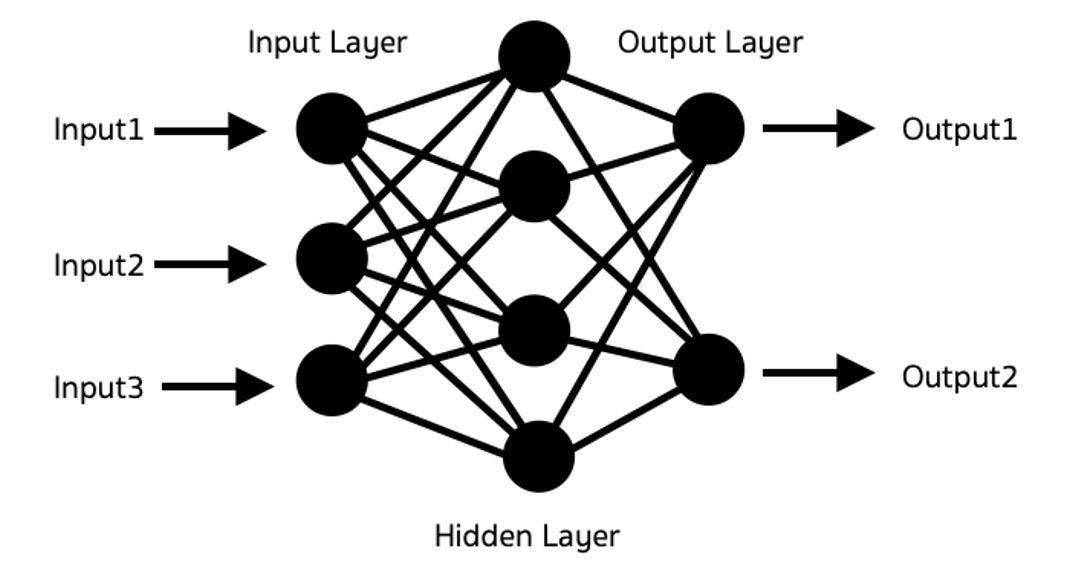
\includegraphics[scale = 0.4]{artificial example.JPG}
    \caption{แสดงโครงสร้างของโครงข่ายประสาทเทียม}
    \label{Fig:artificial_example}
\end{figure}

การหาค่าผิดพลาด (Error) ของโครงข่ายประสาทเทียมจะใช้อัลกอรึทึมที่ชื่อว่า feed-forward neural networks 
คือข้อมูลจะถูกส่งไปข้างหน้าเพียงหนึ่งทิศทางเท่านั้น 
กล่าวคือข้อมูลจะถูกส่งจากชั้นขาเข้าไปยังชั้นซ่อนและส่งต่อไปยังชั้นผลลัพธ์ขาออกเท่านั้นและเมื่อได้ผลลัพธ์ออกมาแล้ว 
จะนำผลลัพธ์ที่ได้มาคำนวณกับค่าเป้าหมายเพื่อหาค่าผิดพลาด 
จากนั้นนำค่าผิดพลาดที่คำนวณได้ไปใช้ในการปรับค่าน้ำหนักของข้อมูล \par

ข้อมูลที่รับเข้ามาจะถูกคูณด้วยค่าน้ำหนัก (Weight) ก่อนจะถูกส่งต่อไปยังเซลล์ประสาทในชั้นซ่อน 
โดยในหนึ่งเซลล์ประสาทในชั้นซ่อนนั้นจะประกอบไปด้วยฟังก์ชันทางคณิตศาสตร์หรือ Activation function 
ที่ใช้ในการพิจารณาผลลัพธ์ดังภาพ~\ref{Fig:Activation_function}

\begin{figure}[h]
    \centering
    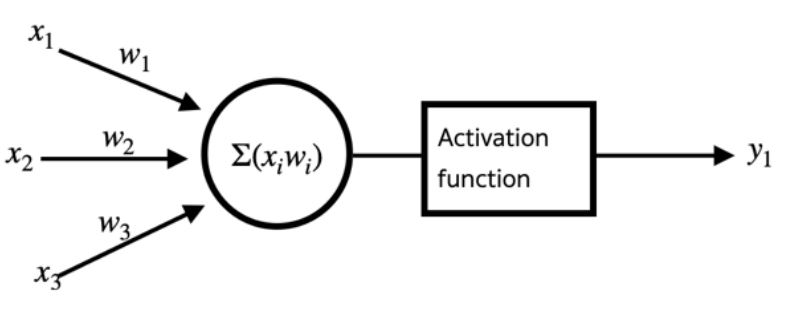
\includegraphics[scale = 0.5]{activation_function.JPG}
    \caption{แสดงการทำงานของเซลล์ประสาทเทียมกับ Activation Function}
    \label{Fig:Activation_function}
\end{figure}

ซึ่ง Activation function ที่เป็นที่นิยมได้แก่ Sigmoid, Softmax และ ReLU Activation Function โดยที่ 
Sigmoid Function จะเป็นการเปลี่ยนผลรวมของข้อมูลที่เข้ามาให้มีค่าอยู่ระหว่าง 0 ถึง 1 เท่านั้น จึงเหมาะที่จะถูกนำไปใช้ในงานที่ต้องการ ผลลัพธ์ หรือ output
ที่เป็นความน่าจะเป็น (Probability) ส่วน Softmax Function จะให้ผลลัพธ์เป็น 0 ถึง 1 เหมือนกันแต่สามารถนำไปใช้งานได้หลากหลายกว่า
เพราะเป็นการแสดงผลลัพธ์ของหลาย ๆ ข้อมูลที่เข้ามารวมกันเป็นหลาย ๆ ผลลัพธ์ซึ่งเหมาะมากกับการนำไปใช้ในการจำแนกประเภทหลายคลาส (Multi-Class Classification) 
ส่วน ReLU Function คือฟังก์ชั่นที่ได้รับความนิยมสูงสุดในขณะนี้ โดยที่ถ้าได้ผลลัพธ์ต่ำกว่า 0 จะได้ผลลัพธ์เป็น 0 โดยทันที
แต่หากได้ค่ามากกว่าหรือเท่ากับ 0 ก็จะได้ผลลัพธ์เป็นค่านั้น ๆ ซึ่ง ReLU นั้นนิยมใช้มากในงานโครงข่ายประสาทแบบคอนโวลูชันและโครงข่ายประสาทเชิงลึก \par

\begin{figure}[h]
    \centering
    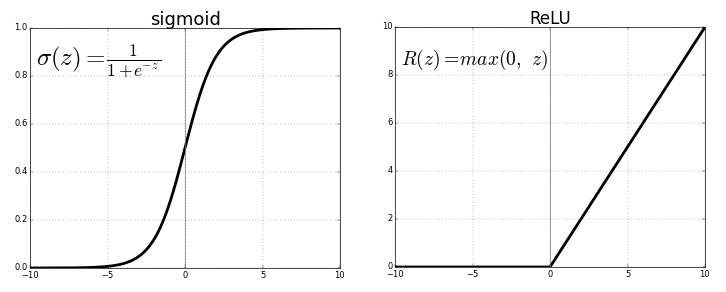
\includegraphics[scale = 0.4]{sigmoin_v_relu.png}
    \caption{รูปเปรียบเทียบระหว่าง Sigmoid และ ReLU Function}
    \label{Fig:Sigmoind_v_Relu}
\end{figure}

\subsection{โครงข่ายประสาทเชิงลึก (Deep Neural Network)} \par
โครงข่ายประสาทเชิงลึกเป็นการต่อยอดมาจากโครงข่ายประสาทเทียม (Artificial Neural Network) และเป็นส่วนหนึ่งที่อยู่ภายใต้ศาสตร์การเรียนรู้ของเครื่อง (Machine Learning)
กล่าวคือในชั้นซ่อนของโครงข่ายประสาทเชิงลึกจะมีจำนวนมากกว่าจำนวนชั้นซ่อนของโครงข่ายประสาทเทียม
และใช้อัลกอริทึมในการปรับค่าน้ำหนักที่ต่างกันด้วย

\begin{figure}[h]
    \centering
    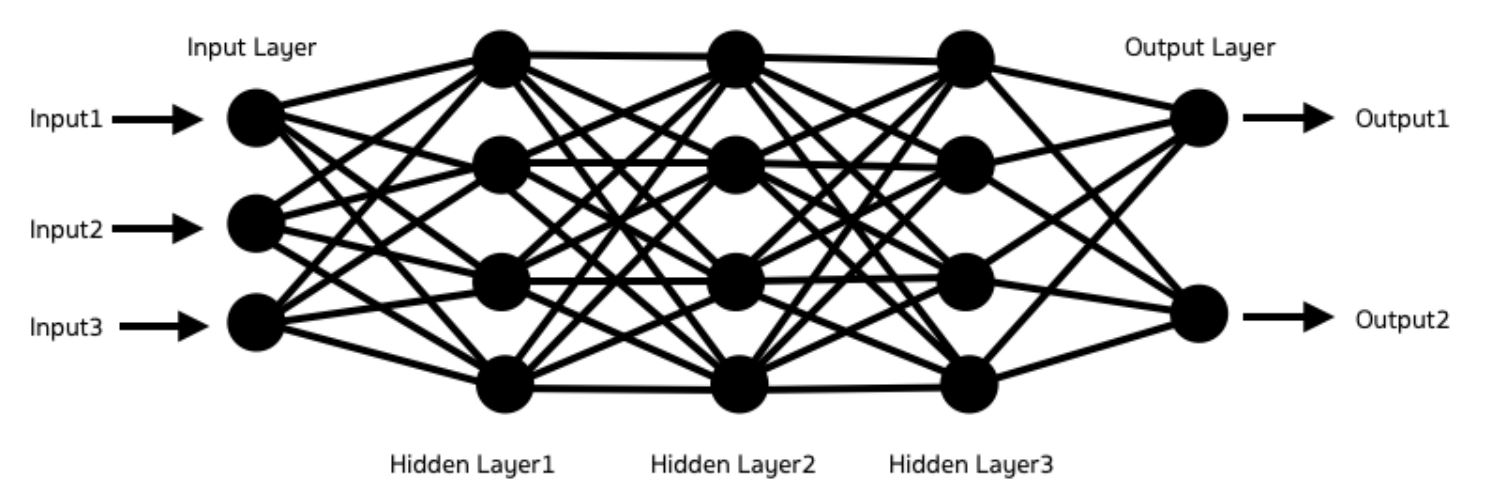
\includegraphics[scale = 0.4]{Deep_neural_ex.JPG}
    \caption{แสดงโครงสร้างของโครงข่ายประสาทเชิงลึก}
    \label{Fig:Deep_neuralnet}
\end{figure}

ในโครงข่ายประสาทเทียมเชิงลึกจะใช้อัลกอริทึม Backward Propagation ในการปรับค่าน้ำหนัก 
ในขั้นแรกจะทำ feed-forward เมื่อเสร็จสิ้นแล้วจะทําการปรับค่าน้ำหนักของโครงข่ายประสาทเทียมเชิงลึกโดยใช้จะใช้อัลกอริทึม 
Backward Propagation และใช้อัลกอริทึม Gradient Descent ในการหาค่าน้ำหนักที่เหมาะสมที่สุด

\begin{itemize}

    \item\textbf{การส่งค่าย้อนกลับ (Backward Propagation or Back Propagation)}

    ก่อนที่จะมีการส่งค่าย้อนกลับนั้น ต้องทำการคำนวณหาค่าผิดพลาด (Error) จากผลลัพธ์ที่ได้มาจากโครงข่ายประสาทเทียมก่อน 
    โดยนําผลลัพธ์ที่ได้จากโครงข่ายประสาทเทียมมาเปรียบเทียบกับผลลัพธ์เป้าหมาย 
    เมื่อได้ค่าผิดพลาดมาแล้วจะทำการส่งค่าผิดพลาดนี้กลับไปยังพารามิเตอร์ที่มีส่วนเกี่ยวข้องหรือก็คือค่าของน้ำหนักนั่นเอง
    เนื่องจากค่าผลลัพธ์ที่ได้จากโครงข่ายประสาทเทียมนั้น ถูกคำนวณมาจากค่าของน้ำหนัก สิ่งที่เราต้องทราบคือค่าน้ำหนักแต่ละตัวนั้นมี
    ผลกระทบต่อค่าผิดพลาดมากน้อยแค่ไหน โดยคำนวณจากการหาอนุพันธ์ของค่าผิดพลาดเทียบกับน้ำหนัก

    \begin{figure}[h]
        \centering
        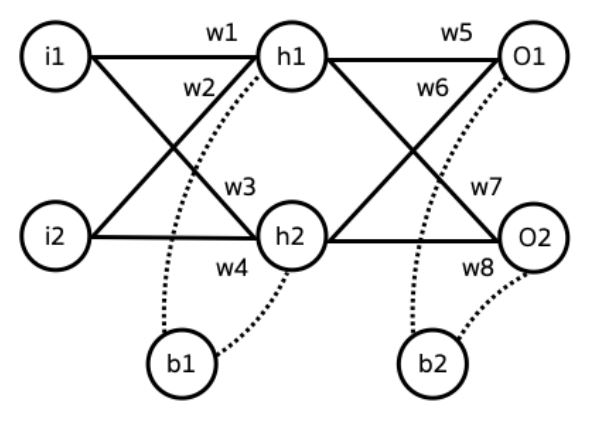
\includegraphics[scale = 0.5]{artificial example_2.JPG}
        \caption{แสดงโครงข่ายประสาทเทียม}
        \label{Fig:Artificial_2}
    \end{figure}

    เพื่อให้ง่ายต่อการอธิบายจึงยกตัวอย่างของโครงข่ายประสาทเทียมดังภาพ~\ref{Fig:Artificial_2} มาช่วยในการอธิบาย
    โดยเซลล์ i คือเซลล์ประสาทเทียมในชั้นขาเข้า เซลล์ h แทนเซลล์ประสาทเทียมในชั้นซ่อน และเซลล์
    O แทนเซล์ประสาทเทียมในชั้นผลลัพธ์ โดยผลลัพธ์ที่ได้จากโครงข่ายประสาทเทียมนี้จะสามารถคํานวณได้ตามสมการตัวอย่าง

    \begin{equation}
        \centering
        O1 = h1 \cdot w_5 + h2 \cdot + w_6 + b_2
        \label{eq:arti_ex_1}
    \end{equation}

    จากสมการ~\ref{eq:arti_ex_1} ทำให้ทราบว่าผลลัพธ์ที่ได้จากเซลล์ผลลัพธ์จะเท่ากับ
    ผลลัพธ์ของเซลล์ในชั้นซ่อนก่อนหน้าคูณด้วยน้ำหนักแล้วบวกด้วยค่าอคติหรือ bias 
    ในทำนองเดียวกันการหาผลลัพธ์ของเซลล์ในชั้นซ่อนจะหาจากค่าของข้อมูลในชั้นขาเข้าคูณด้วยน้ำหนักและบวกด้วยค่าอคติดังสมการ~\ref{eq:arti_ex_2}

    \begin{equation}
        \centering
        h1 = i1 \cdot w_1 + i2 \cdot + w_2 + b_1
        \label{eq:arti_ex_2}
    \end{equation}

    หลังจากที่ทราบค่าในแต่ละเซลล์ผลลัพธ์ O1 และ O2 แล้วจะทำการหาผลรวมของค่าผิดพลาด (Error) จากสมการ~\ref{eq:sum_error}

    \begin{equation}
        \centering
        E_{total} = \sum_{i=1}^{n}\frac{1}{2}(y_{i} - f(x_i))^2
        \label{eq:sum_error}
    \end{equation}

    จากสมการแสดงการคำนวณค่าผิดพลาด โดยที่ $y_{target}$ คือผลลัพธ์เป้าหมายและ $y_{out}$ คือผลลัพธ์ที่ได้จากโครงข่ายประสาทเทียม 
    โดยที่เอาค่าที่ได้จากเซลล์ O1 ไปคำนวณด้วย Activation function แล้วนำมาเปรียบเทียบกับผลลัพธ์เป้าหมาย หลังจากที่ได้ค่าผลรวมความผิดพลาดมาแล้ว 
    เราจะทำการหาอนุพันธ์ของค่าผิดพลาดเทียบกับน้ำหนักทีละตัว เพื่อให้ได้ค่าเกรเดียน (Gradient) ของน้ำหนักเพื่อนำไปใช้ในการปรับน้ำหนักดังสมการ~\ref{eq:gradient_1}

    \begin{equation}
        \centering
        \frac{\partial Error(w)}{\partial W}
        \label{eq:gradient_1}
    \end{equation}

    โดยที่ $E_{total}$ คือผลรวมของค่าความผิดพลาด และ $w_i$ คือน้ำหนักตัวที่ $i$
    และเนื่องจากสมการ~\ref{eq:gradient_1}เป็นสมการเชิงอนุพันธ์ย่อย (Partial Differential) จึงต้องใช้กฎลูกโซ่ (Chain Rule) 
    เข้ามาช่วยในการคำนวณ ตัวอย่างเช่นสมการต่อไปนี้ีจะแสดงการหาอนุพันธ์ระหว่างผลรวมของค่าผิดพลาดกับค่าน้ำหนักตัวที่ 5 ($w5$)

    \begin{equation}
        \centering
        \frac{\partial E_{total}}{\partial w_5} = \frac{\partial E_{total}}{\partial y_{out1}} x \frac{y_{out1}}{\partial O_1} x \frac{\partial O_1}{\partial w_5}
        \label{eq:Error_total_1}
    \end{equation}

    หลังจากที่คำนวณสมการข้างต้นแล้ว จะได้ค่าของเกรเดียนของน้ำหนักตัวที่ 5 หรืออัตราการเปลี่ยนแปลงของน้ำหนักตัวที่
    5 หลังจากนั้นเราจะนำค่าเกรเดียนที่ได้ไปใช้ในการปรับค่า
    น้ำหนักเพื่อที่จะลดค่าผิดพลาดให้มีค่าน้อยที่สุด โดยใช้สมการดังนี้

    \begin{equation}
        \centering
        W_{new} = W_{old} - \alpha *\frac{\partial Error(w)}{\partial W}
        \label{eq:new_weight_1}
    \end{equation}

    โดยที่ $\alpha$ คือค่าอัตราการเรียนรู้ (Learning Rate) เป็นค่าไฮเปอร์พารามิเตอร์ (Hyperparameter) ที่ควบคุมการปรับค่าน้ำหนักของ
    โครงข่ายประสาทเทียมว่ามากหรือน้อยแค่ไหนในหนึ่งขั้นตอน (Step) ของการฝึกอบรมแบบจำลอง ซึ่งเป็นค่าคงที่ 
    และหลังจากทำการปรับน้ำหนักแล้ว จะเริ่มทำการคำนวณแบบเดียวกันกับค่าน้ำหนักตัวอื่น ๆ ในชั้นเดียวกันจนครบทุกตัว ขั้นต่อไปคือการคำนวณในทำนาองเดียวกันกับชั้นก่อนหน้า
    โดยที่จะคำนวณอย่างนี้ซ้ำ ไปจนกระทั่งน้ำหนักทุกตัวได้รับการปรับปรุงจนหมด

\end{itemize}


\subsection{โครงข่ายประสาทแบบคอนโวลูชัน (Convolutional Neural Network, CNN)}
โครงข่ายประสาทแบบคอนโวลูชันเป็นโครงข่ายประสาทเทียมหนึ่งในกลุ่มของ bio-inspired โดยจะจำลองการมองเห็นของมนุษย์ที่จะมองพื้นที่เป็นย่อย ๆ และนำพื้นที่ย่อย ๆ มารวมกันเพื่อดูว่าสิ่งที่มนุษย์มองอยู่นั้นคืออะไร
ซึ่งในการมองพื้นที่ย่อย ๆ ของมนุษย์นั้น จะมีการคัดแยกคุณลักษณะ (Feature Extraction) ของพื้นที่นั้น ๆ เช่นลายเส้น สี การรวมกันของลายเส้นและสี
การมองภาพผ่านดวงตาของมนุษย์นั้นจะแบ่งการมองออกเป็นสองจุดใหญ่ ๆ คือจุดที่โฟกัสหรือสนใจและบริเวณต่าง ๆ โดยรอบของจุดนั้น ๆ  เมื่อนำมาประกอบกันจะทำให้สมองประมวลผลสิ่งที่เห็นและจะทำให้ทราบว่าสิ่ง ๆ นั้นคืออะไร

\begin{figure}[h]
    \centering
    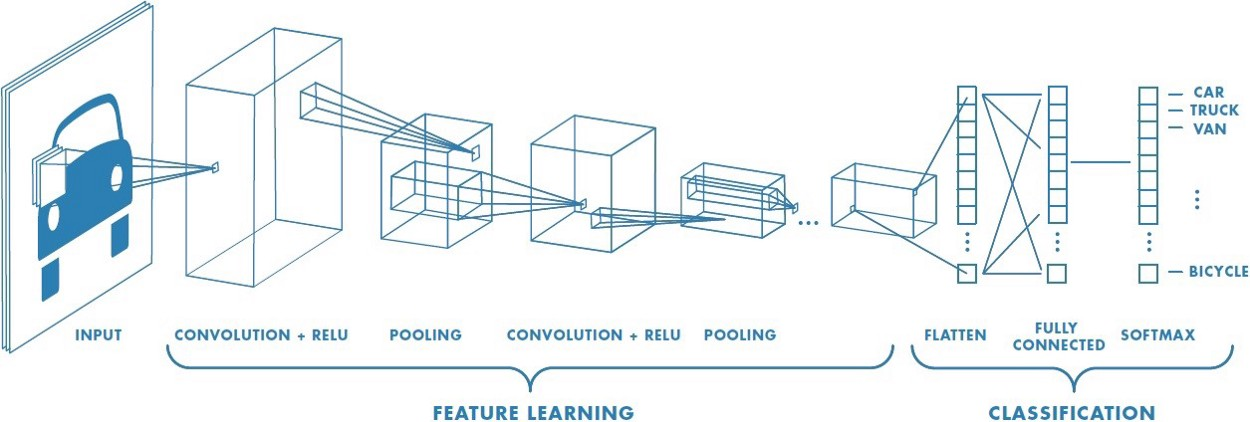
\includegraphics[scale = 0.3]{cnn_1.jpeg}
    \caption{แสดงสถาปัตยกรรมของโครงข่ายประสาทเทียมแบบคอนโวลูชัน}
    \label{Fig:conv_arch_ex1}
\end{figure}

\begin{itemize}

    \item \textbf{การคัดแยกคุณลักษณะเด่น (Feature Extraction) ในโครงข่ายประสาทแบบคอนโวลูชัน} \par
    
    เพื่อให้โครงข่ายประสาทเทียมมีการคำนวณที่สอดคล้องกับแนวคิดของตัวมันเองนั้น 
    จึงมีการนำคณิตศาสตร์เข้ามาช่วยในการคำนวณโดยใช้หลักการเดียวกับ คอนโวลูชันเชิงพื้นที่ (Spatial Convolution) 
    ในงานด้านการประมวลผลภาพดิจิตัล (Digital Image Processing) การคำนวณนี้จะมีการกำหนดค่าของตัวกรอง (Filter) ที่จะช่วยในการดึงคุณลักษณะที่ใช้ในการเรียนรู้และจดจำวัตถุออกมา
    โดยปกติตัวกรองหนึ่งตัวจะดึงคุณลักษณะที่สนใจออกมาได้เพียงหนึ่งคุณลักษณะเท่านั้น ทำให้จำเป็นต้องมีตัวกรองหลายตัวเพื่อหาคุณลักษณะทางพื้นที่หลาย ๆ อย่างมาประกอบกัน
    
    \item \textbf{ลักษณะของตัวกรอง} \par
    
    ตัวกรองสำหรับภาพดิจิตัลนั้นโดยทั่วไปจะเป็นตาราง 2 มิติที่มีขนาดภาพตามพื้นที่ย่อย ๆ ที่ต้องพิจารณา

    \begin{figure}[h]
        \centering
        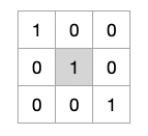
\includegraphics[scale = 0.5]{filter_3x3.JPG}
        \caption{แสดงตัวกรองขนาด 3 X 3}
        \label{Fig:filter_3X3}
    \end{figure}

    โดยที่ช่องที่แรเงาตรงกลางจะถูกเรียกว่า Anchor มีหน้าที่เอาไว้ทาบกับพิกเซลของข้อมูลภาพขาเข้า 
    เริ่มแรกตัวกรองจะถูกวางทาบลงไปบนพิกเซลแรกของข้อมูลภาพ และหลังจากนั้นจะถูกเลื่อนไปในตำแหน่งของพิกเซลถัดไปทีละพิกเซลจนครบทุกพิกเซลในภาพ
    ในขั้นตอนนี้มีข้อจำกัดคือ ตัวกรองจะไม่สามารถถูกนำไปทาบกับพิกเซลที่อยู่ใกล้กับขอบภาพได้ เนื่องจากตัวกรองจะเกินออกไปนอกภาพ เมื่อตัวกรองถูกเลื่อนไปจนครบทุกตำแหน่งที่สามารถเลื่อนไปได้แล้ว สิ่งที่ได้จากขั้นตอนนี้ จะถูกเรียกว่า 
    ผังคุณลักษณะ (Feature Map)

    \item \textbf{การทำคอนโวลูชัน} \par
    
    การทำคอนโวลูชันเป็นการคูณเมทริกซ์ระหว่างข้อมูลภาพขาเข้า กับตัวกรอง เมื่อนำตัวกรองไทาบลงบนข้อมูลภาพขาเข้าแล้ว ค่าในทุก ๆ 
    ตำแหน่งที่ตรงกันจะทำการคูณกัน หลังจากนั้นจะรวมผลลัพธ์ที่ได้ทั้งหมดเข้าด้วยกันในตำแหน่งที่เรียกว่า Anchor หลังจากนั้นจะเลื่อนตัวกรองไปยังตำแหน่งถัดไป 
    เมื่อทำครบทุกพิกเซลแล้วจะได้ผลลัพธ์ที่เป็นผังคุณลักษณะออกมา
    
    \begin{figure}[h]
        \centering
        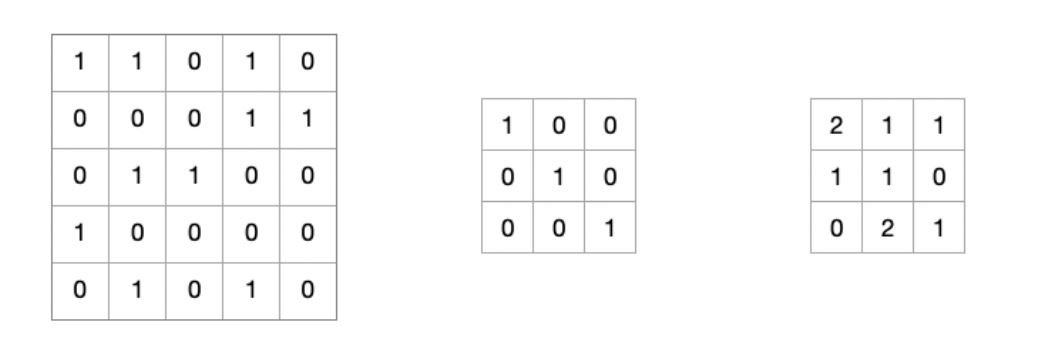
\includegraphics[scale = 0.4]{feature_mapre_1.JPG}
        \caption{แสดงตัวอย่างของข้อมูลภาพขาเข้า ตัวกรอง และผังคุณลักษณะ}
        \label{Fig:input_fil_feature}
    \end{figure}

    \begin{figure}[h]
        \centering
        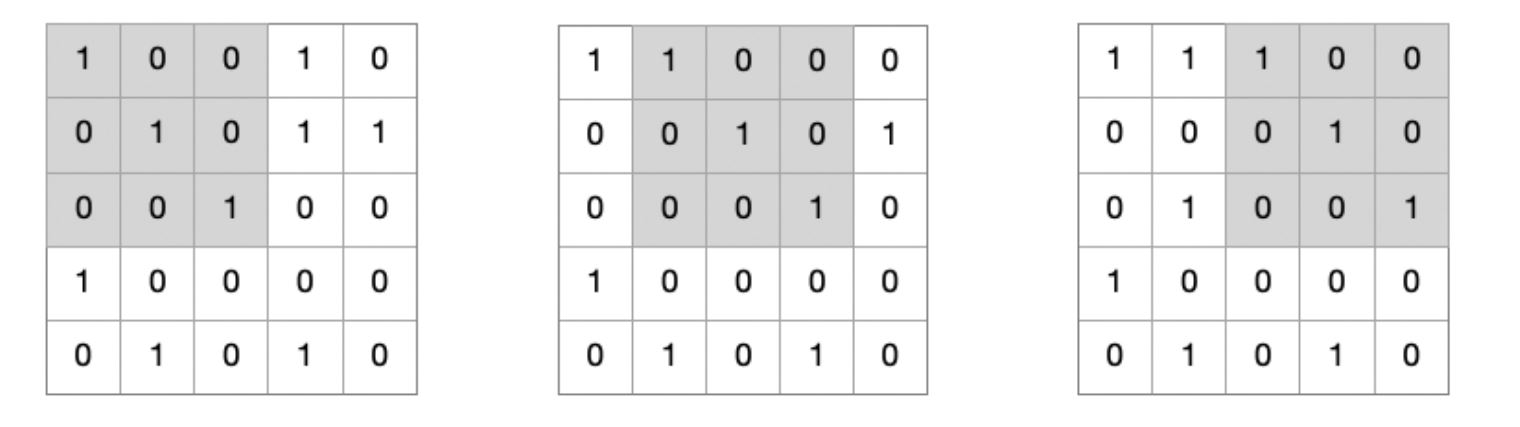
\includegraphics[scale = 0.35]{feature_mapre_2.JPG}
        \caption{แสดงตัวอย่างลักษณะการเคลื่อนที่ของตัวกรองเพื่อให้ได้ผลลัพธ์ดังภาพ~\ref{Fig:input_fil_feature}}
        \label{Fig:feature_stride_eg_1}
    \end{figure}
    
    \item \textbf{Stride และ Padding} \par
    
    \textbf{Stride} เปรียบเสมือนระยะห่างในการเลื่อนพิกเซลของตัวกรอง Stride สามารถกำหนดให้มากขึ้นได้ 
    ถ้าต้องการคำนวณหาคุณลักษณะที่มีพื้นที่ทับซ้อนกันน้อยลง แต่ในขณะเดียวกันเมื่อค่า Stride มากขึ้นผังคุณลักษณะจะมีขนาดเล็กลง

    \begin{figure}[h]
        \centering
        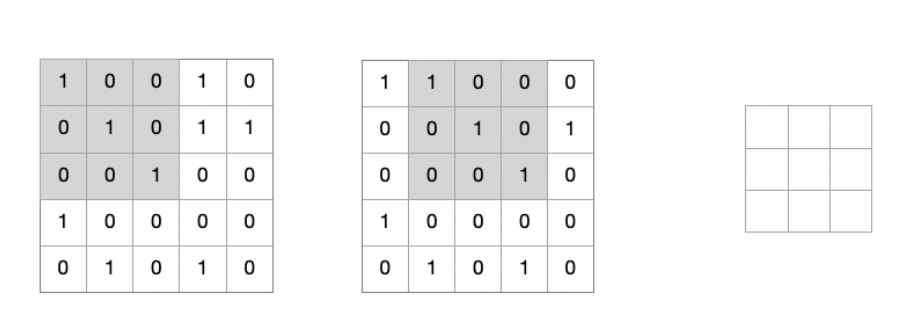
\includegraphics[scale = 0.5]{feature_mapre_3.JPG}
        \caption{แสดงการเคลื่อนที่ของตัวกรองเมื่อ Stride มีค่าเท่ากับ 1 และแสดงผลลัพธ์ของผังคุณลักษณะที่ได้}
        \label{Fig:feature_stride_eg_2}
    \end{figure}
    \begin{figure}[h]
        \centering
        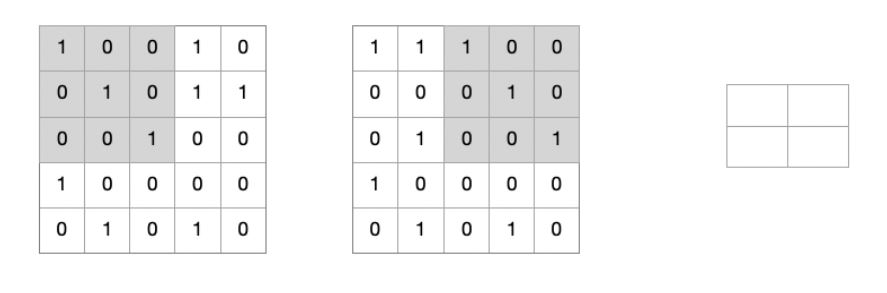
\includegraphics[scale = 0.5]{feature_mapre_4.JPG}
        \caption{แสดงการเคลื่อนที่ของตัวกรองเมื่อ Stride มีค่าเท่ากับ 2 และแสดงผลลัพธ์ของผังคุณลักษณะที่ได้}
        \label{Fig:feature_stride_eg_3}
    \end{figure}
    \FloatBarrier

    \textbf{Padding} จากขั้นตอนการทำคอนโวลูชันที่ผ่านมาจะเห็นได้ว่าผังคุณลักษณะจะมีขนาดเล็กลงกว่าข้อมูลภาพขาเข้า 
    หากต้องการให้ผังคุณลักษณะมีขนาดเท่ากับข้อมูลภาพขาเข้าก็จะต้องมีการเติม 0 หรือค่าต่าง ๆ เข้าไปรอบ ๆ ข้อมูลภาพขาเข้า 
    วิธีนี้จะช่วยแก้ปัญหาในกรณีที่ขอบของภาพมีความสำคัญที่ส่งผลต่อการตัดสินใจดังรูป~\ref{Fig:padding_1}

    \begin{figure}[h]
        \centering
        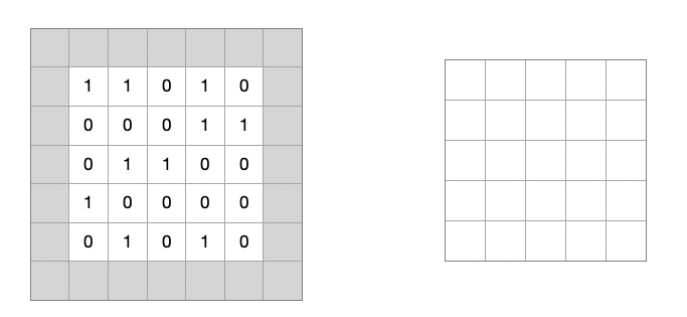
\includegraphics[scale = 0.45]{padding_1.JPG}
        \caption{แสดงข้อมูลรูปภาพที่มีการทำ Padding และแสดงของผังคุณลักษณะที่ได้หลังจากการทำ Padding}
        \label{Fig:padding_1}
    \end{figure}
    
    \item \textbf{Max Pooling} \par
    มนุษย์เราจำแนกวัตถุโดยอาศัยการดูรายละเอียดเล็ก ๆ และมองแบบคร่าว ๆ บนพื้นที่ใหญ่ ๆ จึงทำให้เกิดปัญหาหากต้องใช้ข้อมูลที่หยาบหรือละเอียดอย่างใดอย่างหนึ่งในการจำแนกวัตถุ
    ดังนั้นในการฝึกอบรมแบบจำลองควรมีข้อมูลทั้งหยาบและละเอียดควบคู่กันไป 
    เพื่อให้สามารถจัดการกับปัญหานี้ได้ การย่อขนาดภาพจึงเป็นสิ่งสำคัญ 
    เนื่องจากขนาดของตัวกรองมีความเท่าเดิมอยู่ตลอด 
    ถ้าข้อมูลภาพที่เข้ามามีขนาดใหญ่เราจะได้ข้อมูลที่มีความละเอียดมาก 
    ในขณะเดียวกันถ้าข้อมูลภาพมีขนาดเล็กลง ด้วยตัวกรองขนาดเท่าเดิม
    ตัวกรองจะสามารถครอบคลุมพื้นที่ของวัตถุเดิมได้มากขึ้น Pooling 
    คือความสามารถในการย่อรูปแบบหนึ่งมี 2 ประเภทหลัก ๆ ที่เป็นที่นิยมคือ Max Pooling 
    และ Mean Pooling โดย Max Pooling 
    จะนำค่าที่มากที่สุดที่ตัวกรองทาบทับ อยู่มาเป็นผลลัพธ์ โดยตัวกรองของ Max Pooling 
    จะทำงานในลักษณะเดียวกันกับ ตัวกรองในการทําคอนโวลูชัน โดยทั่วไปในการทํา Max Pooling 
    จะใช้ตัวกรองขนาด 2 x 2 และมี Stride เท่ากับ 2

    \begin{figure}[h]
        \centering
        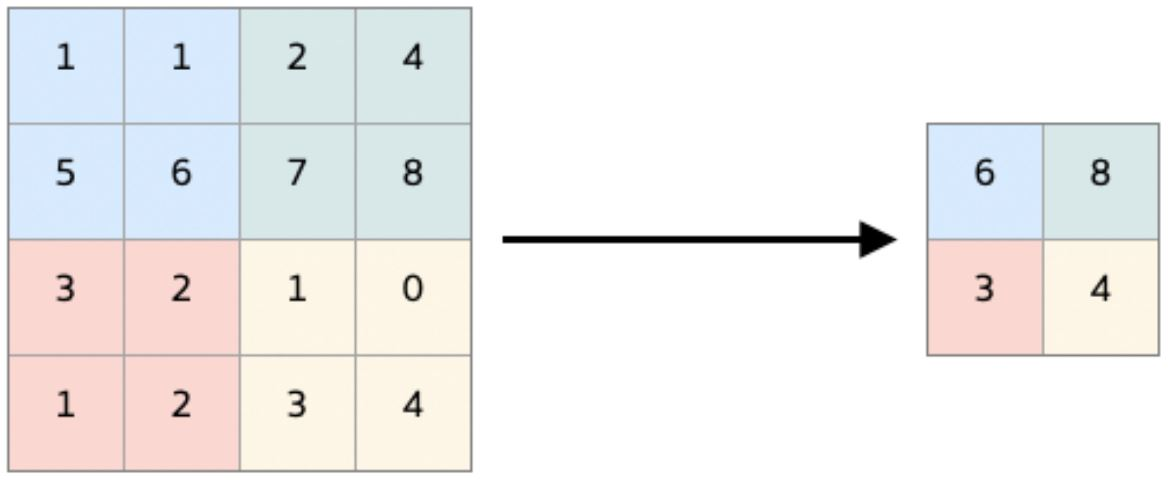
\includegraphics[scale = 0.3]{max_pool_1.JPG}
        \caption{แสดงการทำ Max Pooling ที่มีขนาดตัวกรองเท่ากับ 2 x 2 และ stride เท่ากับ 2}
        \label{Fig:max_pool_1}
    \end{figure}
    
\end{itemize}

\section{สถาปัตยกรรมต่าง ๆ ของโครงข่ายประสาทแบบคอนโวลูชันและการกำหนดองค์ประกอบ (CNN Architecture and Configuration)}


\section{เมตริกที่ใช้ในประเมินผลแบบจำลอง (Evaluation Metrics)}
เมตริกที่ใช้ในการประเมินผลแบบจำลอง โดยปกติแล้วจะมีให้เลือกใช้หลายวิธีด้วยกัน แต่การจะหยิบเมตริกมาใช้ในการประเมินผลแบบจำลองนั้น
จำเป็นจะต้องเลือกวิธีการหรือเมตริกที่เหมาะสมกับอัลกอริทึมของแบบจำลองนั้น ๆ เช่นการวัดความถูกต้องของการแยกประเภท 
(Classification Accuracy)~\cite{international_evalmetric} นั้น คืออัตราส่วนของจำนวนการคาดคะเนที่ถูกต้องต่อจำนวนตัวอย่างอินพุตทั้งหมด 
ซึ่งเรามักจะอ้างอิงถึงความหมายดังที่กล่าวมาข้างต้นตลอดเมื่อเราใช้คำว่า accuracy ในการประเมินผลแบบจำลองในการแยกประเภท
และในบทนี้จะกล่าวถึงเมตริกต่าง ๆ ที่ใช้ในการประเมินผลแบบจำลองว่ามีความหมายอะไร ควรนำเมตริกต่าง ๆ 
ที่ว่า ไปใช้ตอนไหนและจะใช้งานมันอย่างไร ดังนี้


\subsection{F1-Score}
F1-Score คือค่าเฉลี่ยแบบ harmonic mean ระหว่าง precision และ recall โดยนักวิจัยสร้าง F1-Score ขึ้นมาเพื่อเป็น metric แบบตัวเดียวที่สามารถใช้วัดความสามารถของแบบจำลอง ได้โดยไม่ต้องเลือกตัวใดตัวหนึ่งระหว่าง precision  recall และในทางปฏิบัติหากเราจะดูค่า F1-Score, precision หรือ recall เพื่อวัดประสิทธิภาพของแบบจำลอง 
เราควรจะดูค่าเหล่านี้ร่วมกับ ค่าความแม่นยำ (accuracy) เสมอโดยเฉพาะหากเราเจอปัญหากับข้อมูลที่มีสัดส่วนในการจัดกลุ่มไม่เท่ากัน (imbalanced classification)~\cite{Imbalanced_dealing_medium} โดย F1-Score สามารถคำนวณได้จากสมการที่ \ref{eq:f1-score} 
และในส่วนของการคำนวณค่า precision และ recall สามารถคำนวณได้จากสมการ ~\ref{eq:precision} และ ~\ref{eq:recall} ตามลำดับ โดยที่\par

\begin{itemize}
    \item\textbf{True Positive (TP)} คือ จำนวนของผลลัพธ์ที่แบบจำลองทำนายออกมาเป็นบวก (Positive) และผลลัพธ์ที่แท้จริงเป็นบวก (Positive)
    \item\textbf{True Negative (TN)} คือ จำนวนของผลลัพธ์ที่แบบจำลองทำนายออกมาเป็นลบ (Negative) แต่ผลลัพธ์ที่แท้จริงเป็นบวก (Positive)
    \item\textbf{False Positive (FP)} คือ จำนวนของผลลัพธ์ที่แบบจำลองทำนายออกมาเป็นบวก (Positive) แต่ผลลัพธ์ที่แท้จริงเป็นลบ (Negative)
    \item\textbf{False Negative (FN)} คือ จำนวนของผลลัพธ์ที่แบบจำลองทำนายออกมาเป็นลบ (Negative) และผลลัพธ์จริงเป็นลบ (Negative)
\end{itemize}

\begin{equation}
    F1 = 2\times\left(\frac{precision \times recall}{precision  + recall}\right)
    \label{eq:f1-score}
\end{equation}

\begin{equation}
    precision = \frac{TP}{(TP + FP)}
    \label{eq:precision}
\end{equation}

\begin{equation}
    recall = \frac{TP}{(TP + FN)}
    \label{eq:recall}
\end{equation}

\subsection{Receiver Operating Characteristic Curve (ROC Curve)}
ROC Curve คือตัวกราฟแสดงความสัมพันธ์ระหว่างค่า True Positive Rate (TPR) หรือ recall และค่า False Positive Rate (FPR) เพื่อบ่งบอกประสิทธิภาพของการทดสอบแบบจำลองว่า
สามารถแยกผลลัพธ์ที่เป็นบวก (Positive) และเป็นลบ (Negative) ออกจากกันได้ดีแค่ไหน โดย TPR หรือ recall คือค่าที่บอกว่าแบบจำลองของเรานั้นสามารถทำนายผลลัพธ์เป็น positive ได้เป็นอัตราส่วนเท่าไหร่ของค่า positive ทั้งหมด และ FPR คือค่าที่บอกว่าแบบจำลองของเรานั้นสามารถทำนายผลลัพธ์เป็น positive
ได้เป็นอัตราส่วนเท่าไหร่ของค่า negative ทั้งหมดโดยที่ TPR และ FPR สามารถคำนวณได้จากสมการ \ref{eq:TPR} และ \ref{eq:FPR} ตามลำดับ

\begin{equation}
    TPR = recall = \frac{TP}{TP + FN}
    \label{eq:TPR}
\end{equation}

\begin{equation}
    FPR = \frac{FP}{FP + TN}
    \label{eq:FPR}
\end{equation}

\subsection{Area under the ROC Curve (AUC)}
AUC คือ metric ที่บ่งบอกว่าแบบทดลองที่สร้างขึ้นมานั้น สามารถแบ่งแยกความแตกต่างระหว่างผลลัพธ์ที่เป็น 
positive และ negative ได้ดีแค่ไหน ยิ่ง AUC เข้าใกล้ 1 แสดว่าแบบจำลองนั้นสามารถแยก positive และ negative 
ออกได้เป็นอย่างดี ในทางเทคนิค AUC คือพื้นที่ใต้กราฟของ ROC โดยมีตัวอย่างแสดงความสัมพันธ์ของ AUC และ ROC Curve 
ในรูปที่~\ref{Fig:auc_0.4,5789}

\begin{figure}[h]
    \centering
    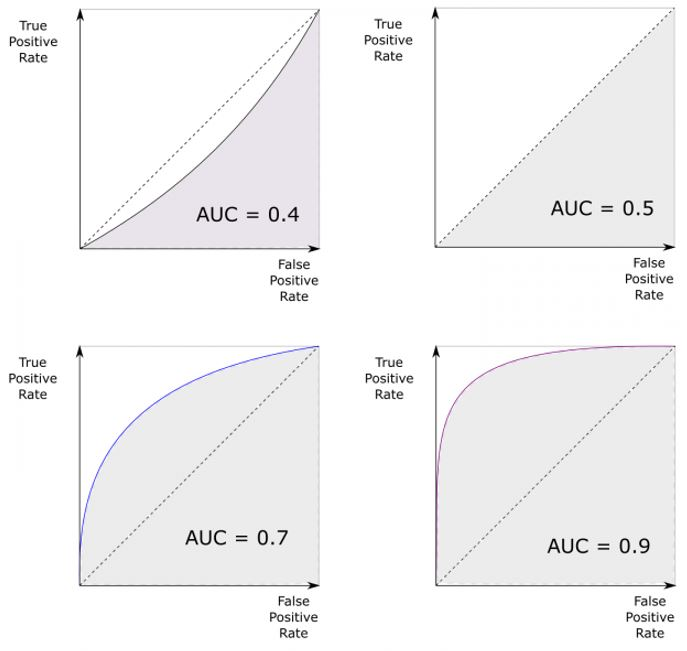
\includegraphics[scale = 0.5]{auc_1.JPG}
    \caption{แสดงความสัมพันธ์ของ AUC และ ROC Curve}
    \label{Fig:auc_0.4,5789}
\end{figure}

\subsection{Mean Average Precision (MAP)}
ในการแข่งขัน BirdCLEF 2020 นี้ทางผู้จัดแข่งขันได้เลือกใช้ metric ตัวนี้เป็นตัววัดและประเมินผลโดย MAP 
คือค่าเฉลี่ยของค่าความแม่นยำเฉลี่ย (Average Precision (AveP)) สามารถคำนวณได้จากสมการ~\ref{eq:MAP}

\begin{equation}
    MAP = \frac{\sum_{q=1}^{Q}AveP(q)}{Q}
    \label{eq:MAP}
\end{equation}

โดย Q คือจำนวนของไฟล์ที่ใช้ในการทดสอบแบบจำลอง และ Avep(q) 
สำหรับไฟล์ q ที่เป็นไฟล์ที่ใช้ในการทดสอบแต่ละไฟล์ซึ่งสามารถคำนวณได้ตามสมการ~\ref{eq:AveP}

\begin{equation}
    AveP = \frac{\sum_{k=1}^{n}(P(k)*rel(k))}{number\, of\, relevant\, document}
    \label{eq:AveP}
\end{equation}


    \chapter{วิธีการดำเนินการวิจัย}
\label{chapter:experiment}

ในส่วนของบทนี้จะพูดถึงลักษณะต่าง ๆ ของข้อมูลเสียงที่ได้ การดำเนินงานในการจัดการกับข้อมูลเสียง 
และสร้างแบบจำลองในแบบต่าง ๆ เพื่อคาดคะเนสายพันธุ์ของนกออกมาเป็นแบบหลายๆฉลาก (multi-label classification) 
ซึ่งลักษณะของข้อมูลเสียงที่ถูกนำมาใช้ในการทดลองและผลงานวิจัยที่เกี่ยวข้องจะถูกพูดถึงในหัวข้อที่ 3.1 
ขั้นตอนการดำเนินงานทั้งหมดจะถูกกล่าวถึงในหัวข้อที่ 3.2 จนถึง หัวข้อที่ 3.4 และจะมีการสรุปผลการศึกษางานวิจัยที่เกี่ยวข้องและ
ขั้นตอนการดำเนินงานทั้งหมดในหัวข้อที่ 3.5

\section{บทนำและงานวิจัยที่เกี่ยวข้อง}
\subsection{การเก็บข้อมูลและลักษณะของข้อมูลเสียง ที่ถูกนำมาใช้ในการทดลอง}
ข้อมูลในส่วนที่ถูกนำมาใช้ ให้เป็นข้อมูลสำหรับการฝึกในครั้งนี้ คือข้อมูลที่มาจากการแข่งขันในปี ค.ศ. 2019~\cite{Kahl2019} แต่ถูกปรับเปลี่ยน 
และพัฒนาคุณภาพขึ้นมาใหม่โดยผู้จัดหาและจัดทำข้อมูลรายใหม่อย่าง Xeno-canto~\cite{xeno-canto}ที่เป็นเว็บไซต์ให้ผู้คนในสาขาต่างๆ ได้ร่วมกันแบ่งปันข้อมูลเสียงนกจากทุกที่ทั่วโลก 
และตัวเว็บไซต์เองไม่ได้เป็นแค่ชุดสะสมการบันทึกเสียงนกเพียงเท่านั้น แต่ยังเป็นโครงงานความร่วมมือที่พร้อมจะให้ทุกคนที่ใช้งานเว็บไซต์มีส่วนร่วมในการช่วยกันแบ่งปันเสียงบันทึกของนก 
และระบุเสียงของนกชนิดต่างๆที่ปรากฏอยู่บนเว็บไซต์ด้วย \par

ข้อมูลจากการแข่งขันเมื่อปี ค.ศ. 2019 นั้น ประกอบไปด้วยทัศนียภาพของเสียงที่ถูกบันทึกด้วยมือกว่า 350 ชั่วโมง ซึ่งโดยส่วนใหญ่ถูกบันทึกไว้ด้วยเครื่องอัดเสียงภาคสนาม 
ช่วงเดือน มกราคม และเดือนมิถุนายน ในปี ค.ศ. 2017 ที่เมืองอิทากา นครนิวยอร์ก ประเทศสหรัฐอเมริกา (Ithaca, NY, USA) และใช้เครื่องบันทึกเสียงรอบทิศทางที่ถูกจัดหาไว้โดยโครงการวิจัยด้านชีวเคมี 
ประจำห้องปฏิบัติการด้านปักษีวิทยา แห่งมหาวิทยาลัยคอร์เนล (Bioacoustics Research Program of the Cornell Lab of Ornithology) 
เครื่องบันทึกเสียงเหล่านี้ สามารถบันทึกเสียงได้มากกว่า 30 หน่วยที่ขยายไปทั้งหมด 1 ตารางไมล์ผ่านแหล่งน้ำที่หลากหลาย และพืชพรรณหลายๆชนิด ซึ่งผู้ติดตั้งและผู้จัดการข้อมูลได้สุ่มเลือก 1 ไฟล์สำหรับแต่ละชั่วโมงในหนึ่งวัน ที่ถูกบันทึกจากเครื่องบันทึก 1 
ใน 30 ตัวที่ถูกติดตั้งไว้ มารวบรวมและบันทึกไฟล์เข้าไว้ด้วยกันเป็นจำนวนทั้งหมด 15 วัน หลังจากนั้นก็นำไฟล์เสียงที่บันทึกไว้มาให้ผู้เชี่ยวชาญ อธิบายและทำเครื่องหมายไว้ว่าแต่ละช่วงเวลาในไฟล์ที่ถูกแบ่งไว้เป็นช่วงๆ ช่วงละ 5 วินาทีนั้น เป็นของนกสายพันธุ์ไหน \par

นอกจากนี้ในตัวชุดข้อมูลเมื่อปี ค.ศ. 2019 ได้มีการหยิบชุดข้อมูลจากการแข่งขัน BirdCLEF เมื่อปี ค.ศ. 2018 กลับมาใช้ซ้ำด้วย ซึ่งเป็นข้อมูลทัศนียภาพของเสียงที่มีความยาวทั้งหมดอยู่ประมาณ 4 ถึง 5 ชั่วโมง ซึ่งข้อมูลดังกล่าวถูกบันทึกที่ประเทศโคลอมเบีย 
โดยนักปักษีวิทยาจากมูลนิธิความหลากหลายทางชีวภาพแห่งโคลอมเบีย ที่มีชื่อว่า Paula Caycedo Rosales และสมาชิกของ Xeno-canto สามารถดูรายละเอียดเกี่ยวกับทัศนียภาพของเสียงโดยรวมได้ที่ หมายเหตุการทำงานของการแข่งขัน BirdCLEF เมื่อปี ค.ศ. 2018~\cite{Goeau2018} \par

ข้อมูลที่ใช้ในการฝึกแบบจำลอง สำหรับการแข่งขัน BirdCLEF ในปีนี้จะประกอบไปด้วยเสียงบันทึกของนกสายพันธุ์ต่างๆที่มาจากทั้งอเมริกาเหนือ อเมริกาใต้ และโซนยุโรป โดยที่ชุมชนของเว็บไซต์ Xeno-canto เป็นผู้จัดหาและสนับสนุนชุดข้อมูลการบันทึกเสียงคุณภาพสูงกว่า 
70,000 การบันทึก ผ่านทางสายพันธุ์นกทั้งหมดกว่า 960 สายพันธุ์ การบันทึกในแต่ละครั้งจะมีเมตาดาต้า (metadata) ประกอบไปกับการบันทึกด้วย โดยในเทตาดาต้าจะประกอบไปด้วย 
สถานที่ในการเก็บบันทึก เวลา และคำอธิบายอื่นๆที่ถูกจัดไว้ให้โดยผู้บันทึกเสียงในการบันทึกครั้งนั้นๆ \par


ส่วนข้อมูลที่จะถูกนำไปใช้ในการทดสอบแบบจำลอง จะประกอบไปทัศนียภาพของเสียงโดยรอบกว่า 153 เสียงที่ถูกบันทึกไว้ในประเทศเปรู สหรัฐอเมริกา และประเทศเยอรมนี โดยในแต่ละเสียงที่ปรากฏ 
จะมีระยะเวลาทั้งหมด 10 นาทีและมีการเปล่งเสียงของนกที่ทับซ้อนกันภายในแต่ละช่วงเวลาในปริมาณที่ค่อนข้างสูง

\subsection{พฤติกรรมการส่งเสียงร้องของนก}
นกใช้เวลาส่วนใหญ่ไปกับการส่งเสียงร้อง แต่ในขณะเดียวกันเสียงร้องของนกในแต่ฤดูกาลจะมีความแตกต่างกัน วัตถุประสงค์ในการส่งเสียงร้องของนกแบ่งออกเป็น 2 อย่างหลัก ๆ ประการแรกคือ นกเพศผู้จะส่งเสียงร้องเพื่อบ่งบอกถึงอาณาเขตของตนเอง 
และประกาศให้ศัตรูรับรู้ว่าจะปกป้องอาณาเขตของตนเองจากเผ่าพันธุ์อื่น ส่วนวัตถุประสงค์ที่สองคือ นกจะส่งเสียงร้องเพื่อดึงดูดคู่ครองและสร้างรัง นกเพศเมียมักจะเลือกคู่ครองโดยขึ้นอยู่กับการผสมผสานระหว่างการมองเห็นและเสียงร้อง 
แม้แต่นกเพศผู้ที่มีขนที่สวยงามในฤดูผสมพันธ์ ก็มีปัญหาในการหาคู่ครองเนื่องจากเสียงร้องที่ไม่สามารถเข้ากันได้ นกแต่ละสายพันธุ์จะมีเสียงร้องเป็นเอกลักษณ์ของตัวเอง 
ทำให้เมื่อนกได้ยินเสียงร้องจะสามารถแยกได้ว่าเสียงร้องนั้นมาจากสายพันธุ์ของตนเองหรือไม่ ถึงแม้ว่านกจะใช้เวลาและพลังงานส่วนใหญ่ไปกับการส่งเสียงร้อง แต่ก็ไม่สามารถทำได้ตลอดทุกฤดูกาล 
โดยส่วนใหญ่จะส่งเสียงร้องมากที่สุดในระหว่างฤดูการทำรังและเมื่อฤดูทำรังสิ้นสุดลงนกจะส่งเสียงร้องน้อยลงและอาณาเขตของพวกมันจะพังทลายลงเนื่องจากมีนกหลายชนิดที่จะทำการอพยพตามฤดูกาล ในนกหลายสายพันธุ์จะมีเพียงเพศผู้ที่ส่งเสียงร้องเท่านั้น 
แต่นอกเหนือจากนั้นนกจะส่งเสียงร้องทั้งเพศผู้และเพศเมีย และในนกบางตัวจะไม่มีการส่งเสียงเลย เช่นอีแร้งและนกกระสาที่แทบจะไม่สามารถสร้างเสียงใด ๆได้~\cite{EarthSky}
ในการระบุสายพันธุ์ของนกด้วยเสียงร้องสามารถสังเกตุได้จากคุณลักษณะของเสียงร้องที่แตกต่างกัน 7 คุณลักษณะ~\cite{Birdingbyear} ดังต่อไปนี้ 

\begin{itemize}
    \item \textbf{ระดับเสียง (Pitch)} เสียงร้องมีความสูงหรือต่ำแค่ไหน?
    \item \textbf{คุณภาพของเสียง (Quality)} มีเสียงที่แตกต่างกันในเสียงร้องหรือไม่? 
    \item \textbf{ความยาว (Length)} เสียงร้องมีความยาวเท่าไหร่? ใช้เวลาเท่าไหร่ในการร้องซ้ำ
    \item \textbf{ความเร็วเพลง (Tempo)} เสียงร้องมีกี่จังหวะ เร็วแค่ไหน? หรือช่วงไหนของเสียงร้องมีการหยุดชั่วคราว
    \item \textbf{ความดังของเสียง (Volume)} เสียงร้องมีการเปลี่ยนระดับความดังหรือไม่? ถ้ามีการเปลี่ยนระดับความดังของเสียง เปลี่ยนที่ตำแหน่งใดและเปลี่ยนอย่างไร? นกที่มีเสียงร้องคล้ายกันแต่ต่างชนิดกันจะมีความดังของเสียงที่ต่างกัน
    \item \textbf{การทำซ้ำ (Repetition)} มีพยางค์ของเสียงที่เหมือนกันซ้ำกันหลายครั้งหรือไม่ ซ้ำกันกี่ครั้ง และมีลำดับที่คล้ายกันเป็นส่วนหนึ่งของเสียงร้องเท่าไหร่?
    \item \textbf{การจำลอง (Mimicry)} มีเสียงที่ผิดปกติที่คล้ายสิ่งอื่นในเสียงร้องหรือไม่ เช่น เสียงสัญญาณกันขโมย เสียงเครื่องมือต่าง ๆ เนื่องจากอาจมีการเลียนแบบเสียงร้องของนก
\end{itemize}

\subsection{กระบวนการขั้นพื้นฐาน (Baseline methods)}
วิธีพื้นฐานที่ใช้กันทั่วไปในการสืบค้นเสียงมีพื้นฐานมาจากพลังงานอย่างใดอย่างหนึ่ง ไม่ว่าจะเป็นคลื่นสเปคตรัมข้ามสหสัมพันธ์ (spectrogram cross-correlation) แบบจำลองมาร์คอฟซ่อนเร้น (Hidden Markov model (HMM))~\cite{Yoon2009} ซึ่งกระบวนการพื้นฐานที่กล่าวมานี้มักเป็นที่รู้จักและ
ใช้กันทั่วไปในการทำวิจัยเกี่ยวกับเสียงสะท้อนชีวภาพ (bioacoustics) \par
แต่ในบางครั้งวิธีที่ง่ายที่สุดมักเป็นการตั้งค่าจุดเปลี่ยนผ่านหากค่าผลลัพธ์ที่ได้ มีค่าสูงกว่าค่าที่ตั้งไว้ (thresholding) ซึ่งจะมีผลลัพธ์เป็นบวก (positive) หากค่าพลังงานในช่วงเวลาสั้นๆที่ตัดมานั้นมีค่าสูงกว่าค่าที่ตั้งไว้
และนอกจากนั้นจะเป็นค่าลบ (negative) และสำหรับการทำเสียงสะท้อนชีวภาพมักจะมีการจัดการกับเสียงรบกวน และการเพิ่มชุดข้อมูล (data augmentation) เพื่อประมาณค่าของเสียงรบกวนที่ได้มาเมื่อเวลาผ่านไป 
และเพื่อให้มั่นใจว่าสามารถรับมือกับเสียงรบกวนได้ตลอด \par
นอกเหนือจากนี้แล้วการจัดแข่ง BirdClef ประจำปีค.ศ. 2018 ได้ให้ตัวอย่างลำดับการทำงานคร่าว ๆ ในการจัดการกับเสียงนกที่ใช้ในการแข่งขันมาเป็นระบบในการตรวจจับเสียงนกแบบพื้นฐาน (Baseline system)~\cite{Kahl2018}
เพื่อให้ผู้เข้าแข่งขันสามารถนำระบบพื้นฐานที่ได้ไปพัฒนาระบบขึ้นมาใหม่เพื่อให้ได้ผลลัพธ์ที่ดีขึ้น โดยระบบพื้นฐานในการตรวจจับเสียงนกที่ผู้จัดแข่งขันให้มานั้นได้ระบุถึงลำดับการทำงาน (Workflow) รายละเอียดชุดข้อมูลสถาปัตยกรรมโครงข่ายประสาทแบบคอนโวลูชัน (CNN Architecture)
การประเมินผล และแนวทางในการพัฒนาระบบต่อไปด้วย

\section{การจัดเตรียมการทดลอง}
ข้อมูลที่ได้จากการแข่งขันในรอบปี ค.ศ. 2020 นี้ได้แบ่งไว้เป็นข้อมูล 3 ชุดหลักๆคือ ข้อมูลที่ใช้สำหรับการฝึกแบบจำลอง (training data) ข้อมูลที่ใช้สำหรับการทดสอบประสิทธิภาพของแบบจำลองเพื่อหา Hyperparameter ที่ดีที่สุด (validation data) และข้อมูลที่ไว้ใช้สำหรับการทดสอบแบบจำลอง (test data) ซึ่งก่อนที่จะสามารถสร้างแบบจำลอง
หรือทำนายผลออกมาได้อย่างสมบูรณ์ก็ต้องมีการ ทำความเข้าใจตัวชุดข้อมูล และจัดเตรียมข้อมูลก่อนนำข้อมูลเข้าให้ดีก่อน
\subsection{การสำรวจชุดข้อมูลเสียงนก (Data exploration)}
จาการสำรวจข้อมูลในเบื้องต้นพบว่าข้อมูลถูกแบ่งออกเป็น 3 ส่วนใหญ่ ๆ โดยมีลายละเอียดดังต่อไปนี้

\begin{itemize}
    \item \textbf{Audio Training Set} ข้อมูลชุดข้อมูลนี้เป็นชุดข้อมูลที่ความไม่สมดุลกันของข้อมูลและข้อมูลชุดนี้ประกอบไปด้วยไฟล์เสียงของนกทั้งหมด 961 สายพันธุ์โดยมีไฟล์เสียงนกทั้งหมด 72324 ไฟล์โดยจัดเก็บนกแต่ละสายพันธุ์ไว้ด้วยโฟลเดอร์ดังที่แสดงในรูป \ref{Fig:folder} และเก็บไฟล์เสียงของนกแต่ละสายพันธุ์จะถูกจัดเก็บไว้ในโฟลเดอร์ที่เก็บไฟล์ .mp3 หลายๆไฟล์ดังที่แสดงในรูป \ref{Fig:filemp3}
    \begin{figure}[h]
        \centering
        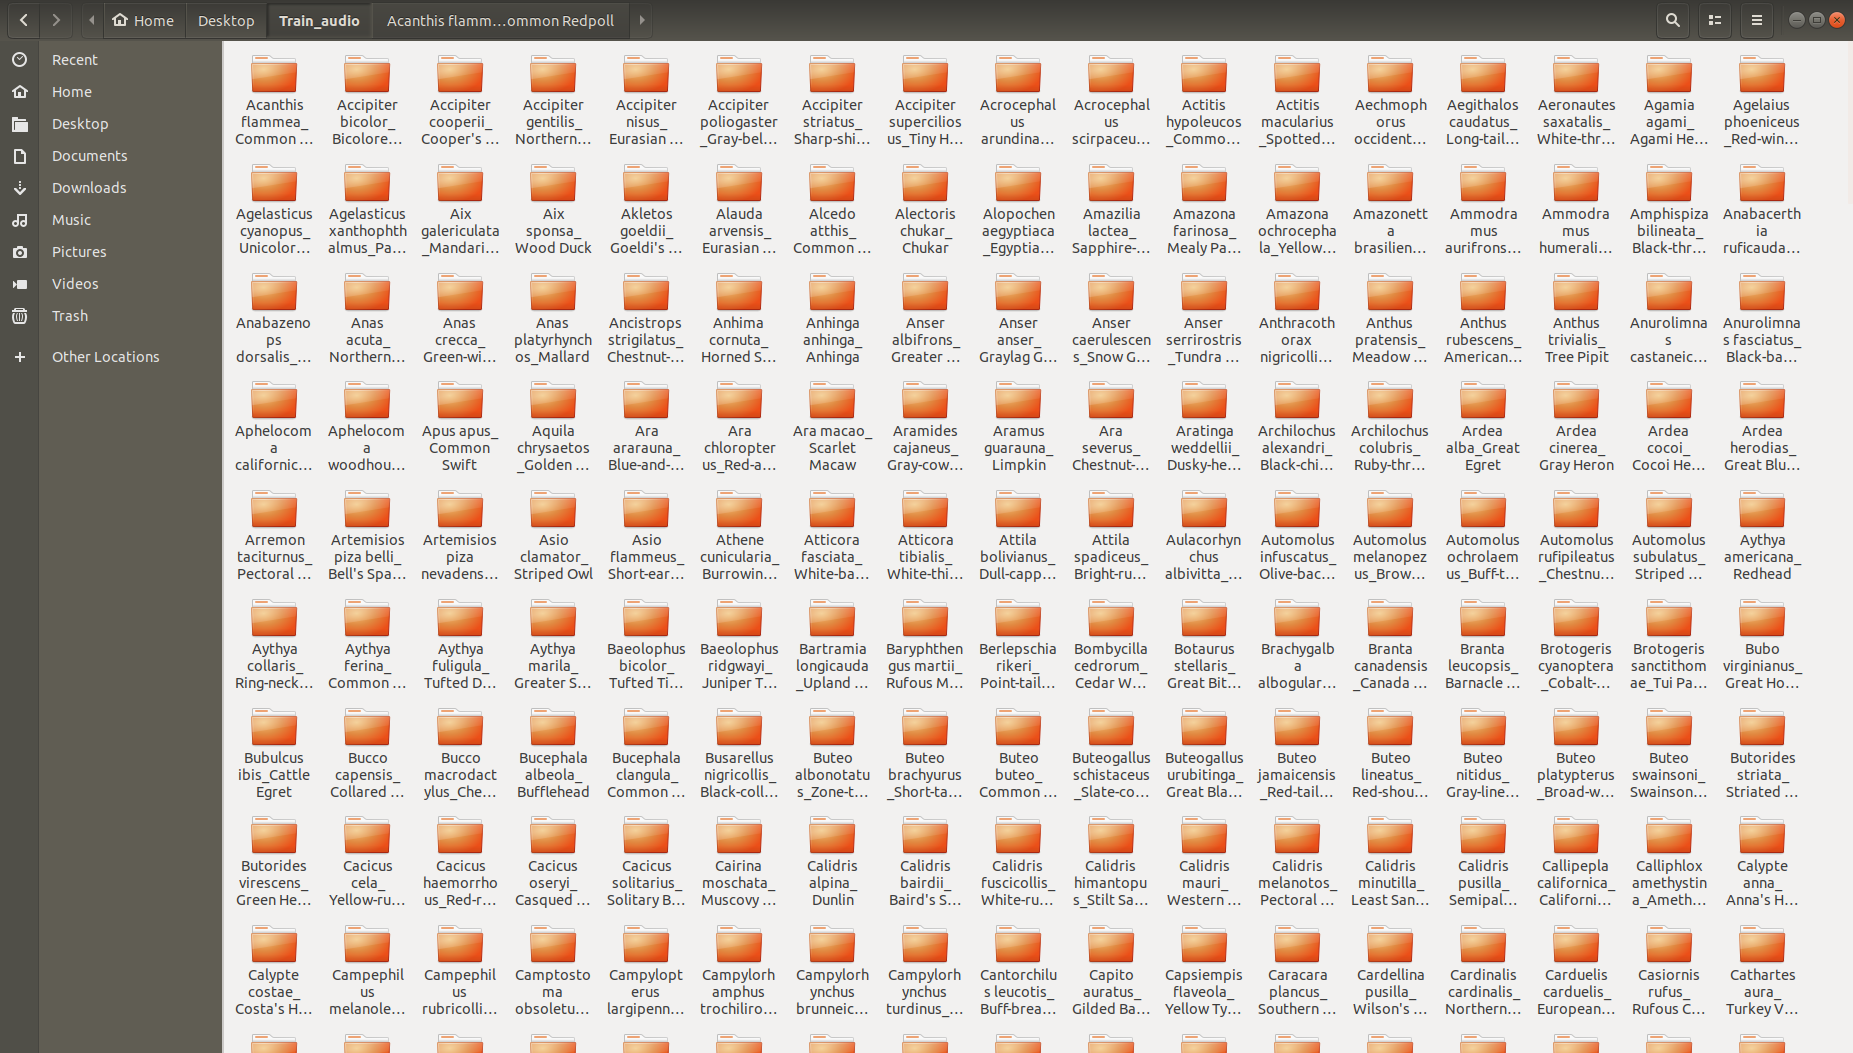
\includegraphics[scale = 0.15]{folder.png}
        \caption{โฟล์เดอร์ที่ใช้ในการเก็บไฟล์เสียง}
        \label{Fig:folder}
    \end{figure}
    \begin{figure}[h]
        \centering
        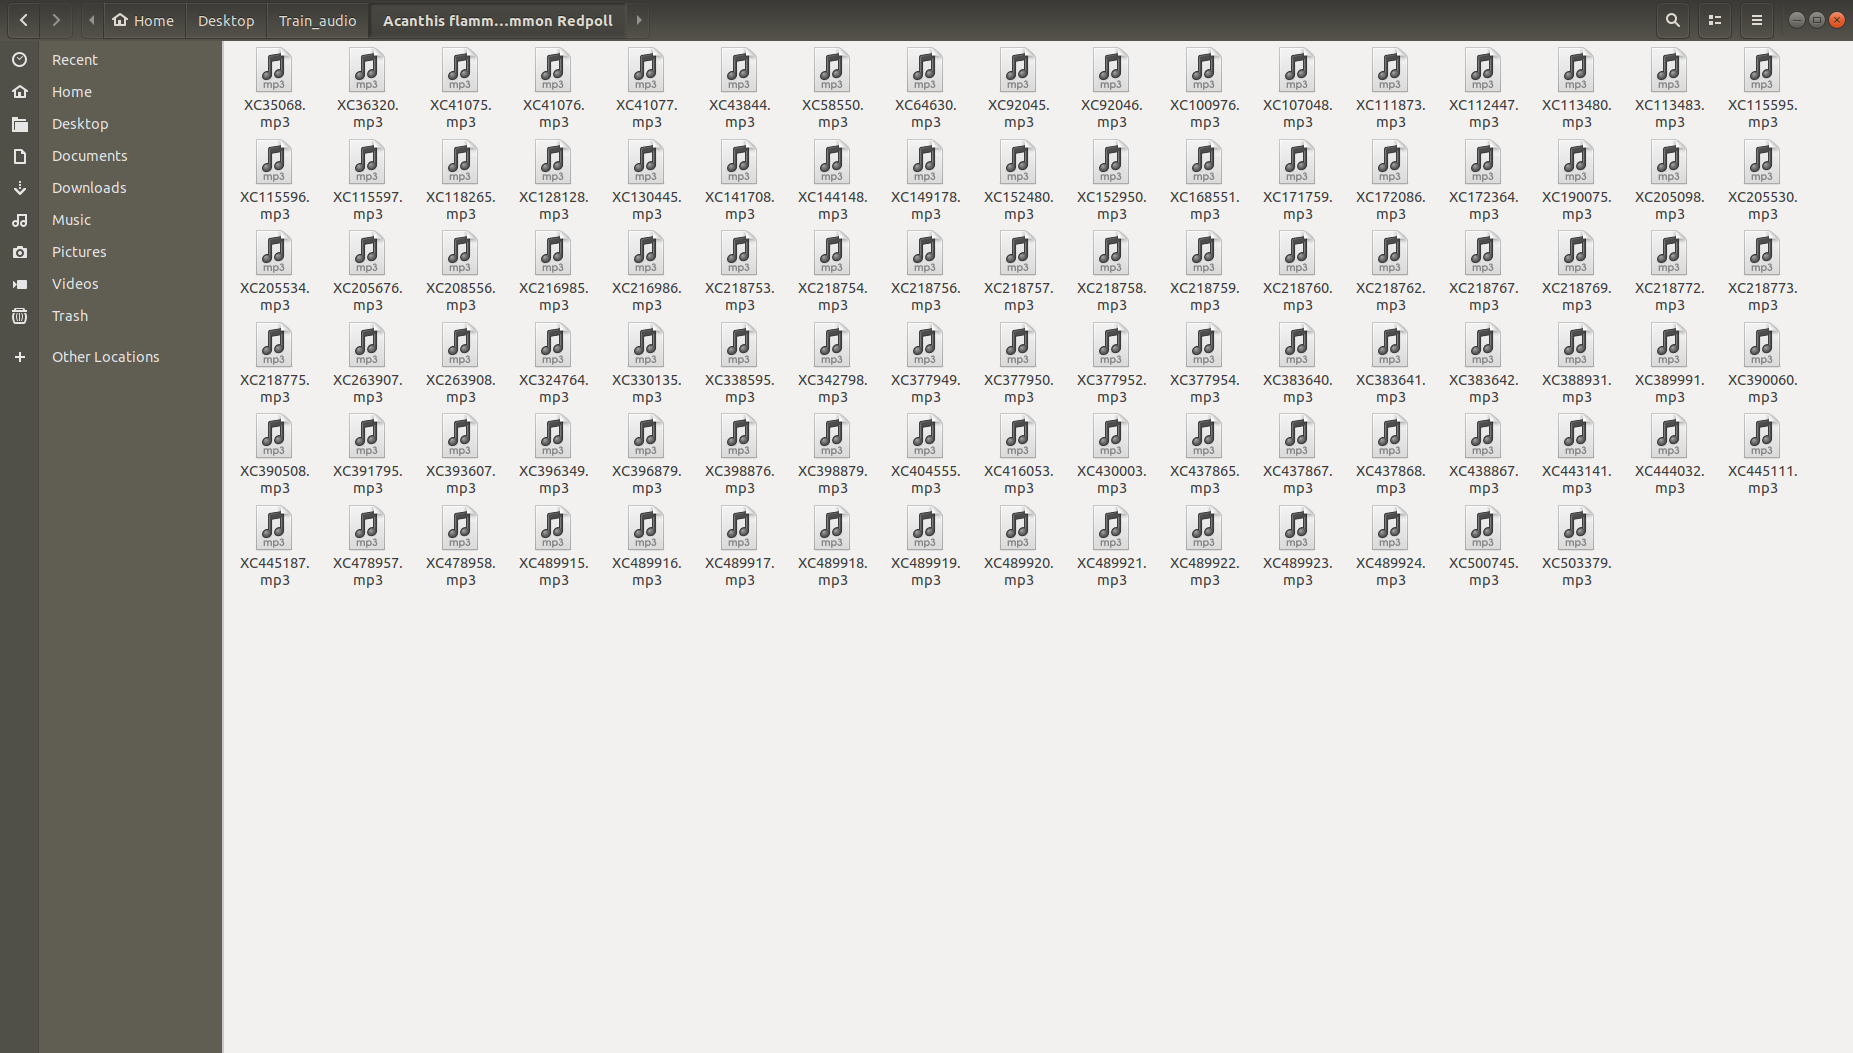
\includegraphics[scale = 0.15]{filemp3.png}
        \caption{ตัวอย่างไฟล์เสียงที่ถูกเก็บไว้ในโฟร์เดอร์}
        \label{Fig:filemp3}
    \end{figure}
    \FloatBarrier

    \item \textbf{Audio Validation set} ข้อมูลชุดนี้คือข้อมูลที่ใช้ในการทดสอบแบบจำลองเพื่อหาค่า Hyperparameter ที่ดีที่สุด โดยข้อมูลในชุดนี้ประกอบไปด้วยข้อมูลเสียงที่เป็นไฟล์ .wav ทั้งหมด 12 ไฟล์ ซึ่งไฟล์เหล่านี้จะถูกนำเข้าไปประมวลผลในแบบจำลองและทำนายว่าเสียงของนก ณ ช่วงเวลานั้น 
    เป็นเสียงของนกสายพันธุ์ใด และอีกส่วนคือไฟล์ข้อมูลที่เป็นไฟล์ .csv ซึ่งทั้งหมด 12 ไฟล์ซึ่งเป็นไฟล์เฉลยสำหรับการทำนายที่ได้จากแบบจำลอง ดังที่แสดงในรูป \ref{Fig:validate} โดยในช่องแรกจะเป็นช่องที่แสดงถึงช่วงเวลาของที่อยู่ภายในไฟล์เสียงนั้นๆ และช่องที่สองคือช่องที่บอกว่าในแต่ละช่วงเวลานั้นเสียงที่ได้ยินคือเสียงของนกสายพันธุ์อะไรแล้วจึงนำค่าที่ได้จากการทดสอบแบบจำลองไปปรับเปลี่ยนการตั้งค่า และหาค่า Hyperparameter ใหม่ให้กับแบบจำลองตามความเหมาะสม
    \item \textbf{Audio Test set} คือชุดข้อมูลที่ไว้ใช้สำหรับทดสอบแบบจำลองที่ประกอบไปด้วยไฟล์เสียง .wav รวมอยู่ทั้งหมด 153 ไฟล์ที่เป็นไฟล์ทัศนียภาพของเสียง โดยแต่ละไฟล์จะมีความยาวอยู่ที่ไฟล์ละ 10 นาที ซึ่งเราต้องนำแบบจำลองของเราไปประมวลผลผ่านไฟล์ที่ได้เพื่อให้ได้คำตอบออกมาดังรูปที่ \ref{Fig:validate} และนำไฟล์คำตอบเหล่านั้นส่งไปยังเว็บไซต์ [21] ที่ผู้จัดแข่ง BirdCLEF 2020 เป็นคนกำหนด
    \begin{figure}[h]
        \centering
        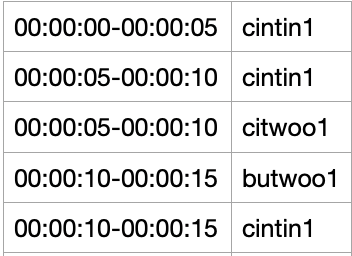
\includegraphics[scale = 0.7]{validation.png}
        \caption{ไฟล์เฉลยการทำงานของแบบจำลอง}
        \label{Fig:validate}
    \end{figure}
    \FloatBarrier
\end{itemize}




% จากกราฟสามารถสรุปชื่อและจำนวนที่พบของนก 6 
% สายพันธุ์ที่พบมากที่สุดในชุดข้อมูลทดสอบประสิทธิภาพของแบบจำลองได้ดังตารางที่ 3.1

% \begin{table}[ht]
%     \centering
%     \caption{แสดงชื่อและจำนวนของนกที่พบมากที่สุด 6 สายพันธุ์}
    
%     \begin{tabular}{|l|c|c|} \hline
%     \multicolumn{1}{|c|}{ชื่อสายพันธ์ุ} & รหัสสายพันธุ์ & จำนวนที่พบ \\ \hline
%     Turdus hauxwelli\_Hauxwell's Thrush   & hauthr1 & 218 \\  \hline
        
%     \end{tabular}
% \end{table}

\subsection{Metrics ที่ใช้สำหรับการประเมินประสิทธิภาพของแบบจำลอง}

    \chapter{ผลการทดลอง}
\label{chapter:result}

ผลลัพธ์การทดสอบประสิทธิภาพในวิธีการใหม่ของเราและเปรียบเทียบกับงานวิจัยอื่น ๆ ที่เกี่ยวข้อง แสดงในตารางที่~\ref{Table:ExperimentalResults} จากตารางดังกล่าว วิธีการของเราได้รับ F-measure สูงที่สุด ที่ 0.506 ซึ่งแสดงให้เห็นชัดเจนว่าวิธีการของเรามีประสิทธิภาพดีกว่าวิธีการ SWT ต้นฉบับ~\cite{5540041} ยิ่งไปกว่านั้นวิธีการของเรายังได้รับ F-meaure ที่มากกว่าวิธีการ BG+ImN~\cite{7532890} และ BG+I2V~\cite{7532890} ซึ่งทั้งสองวิธีนี้ใช้เทคนิค Deep Learning เป็นส่วนหนึ่งในการตรวจหาข้อความในภาพ อย่างไรก็ดีค่า Precision และ Recall สูงสุดของการทดลองนี้อยู่ที่ 0.715 และ 0.481 เป็นของ BG+I2V และ BG+ImN ตามลำดับ สำหรับตัวอย่างพื้นที่ของข้อความที่วิธีการใหม่ของเราตรวจพบถูกแสดงในภาพ~\ref{Fig:ExampleResult}

\begin{table}[!h]    
    \centering
    \begin{tabular}{lccc}
        \hline
        Method & Precision & Recall & F-measure \\ \hline \hline
        STD~\cite{6628665} & 0.165 & 0.051 & 0.078 \\
        SBD~\cite{6761596} & 0.180 & 0.102 & 0.130 \\
        TLD~\cite{rigaud:hal-00841492} & 0.095 & 0.095 & 0.095 \\
        BG + ImN~\cite{7532890} & 0.451 & \textbf{0.481} & 0.466 \\
        BG + I2V~\cite{7532890} & \textbf{0.715} & 0.191 & 0.301 \\
        Baseline~\cite{5540041} & 0.068     & 0.336 & 0.113 \\
        วิธีการของเรา & 0.564     & 0.458 & \textbf{0.506} \\ \hline
    \end{tabular}
    \caption{ตารางแสดงการเปรียบเทียบประสิทธิภาพของวิธีการใหม่ของเราร่วมกับวิธีการอื่น ๆ ที่เกี่ยวข้อง}
    \label{Table:ExperimentalResults}
\end{table}


\begin{figure}[!h]
    \centering
    \subfigure[]{
        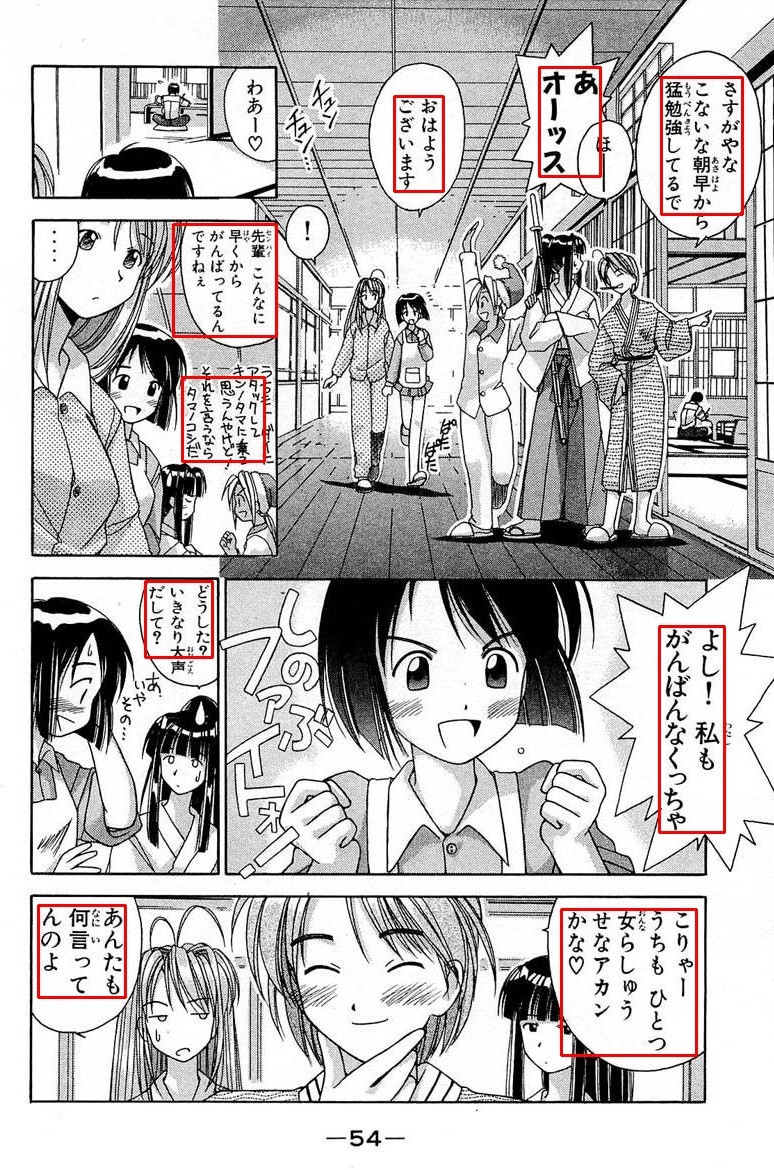
\includegraphics[width=0.45\textwidth]{images/result1.jpg}  
    }
    \subfigure[]{
        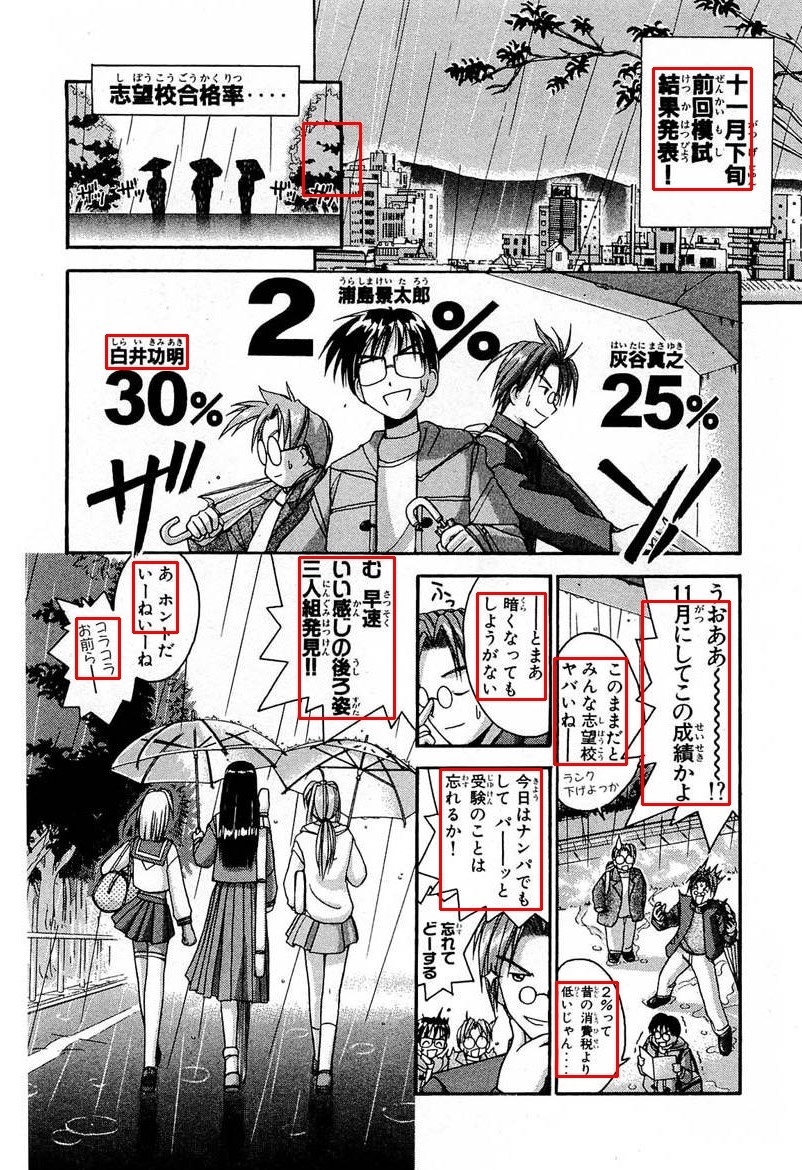
\includegraphics[width=0.45\textwidth]{images/result2.jpg}  
    }
    \subfigure[]{
        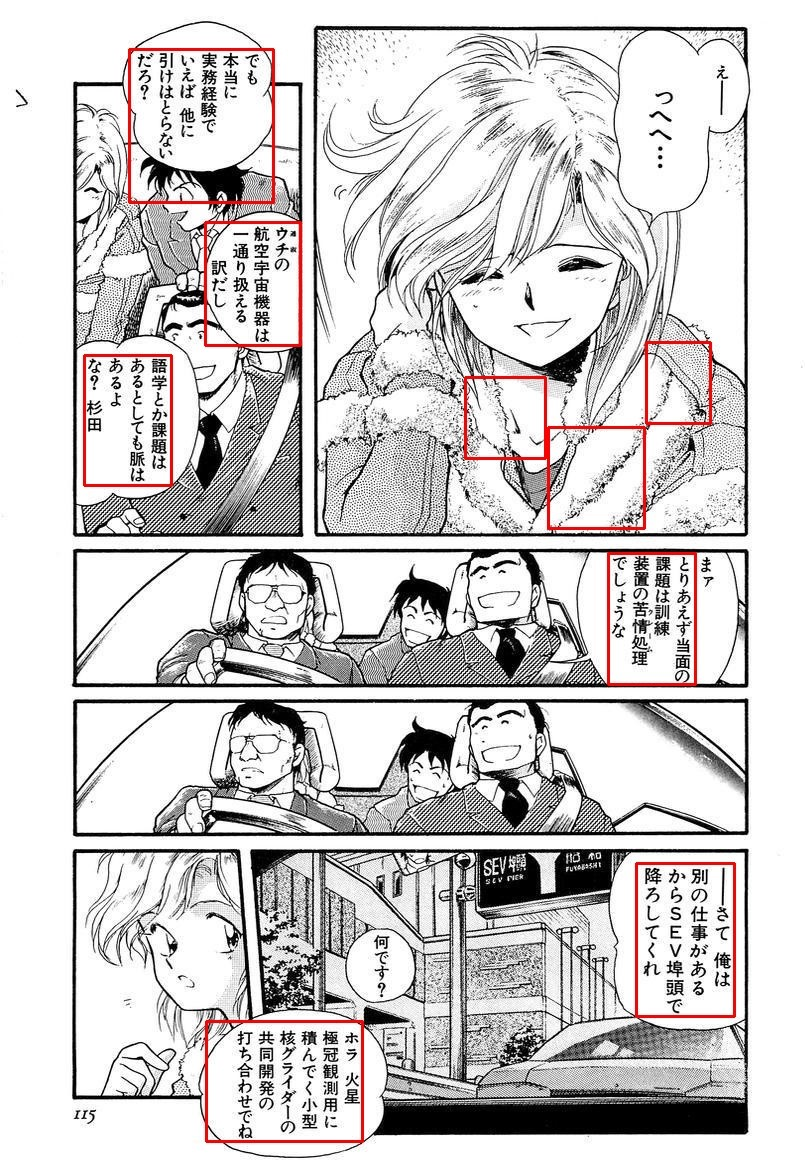
\includegraphics[width=0.45\textwidth]{images/result3.jpg}  
    }
    \subfigure[]{
        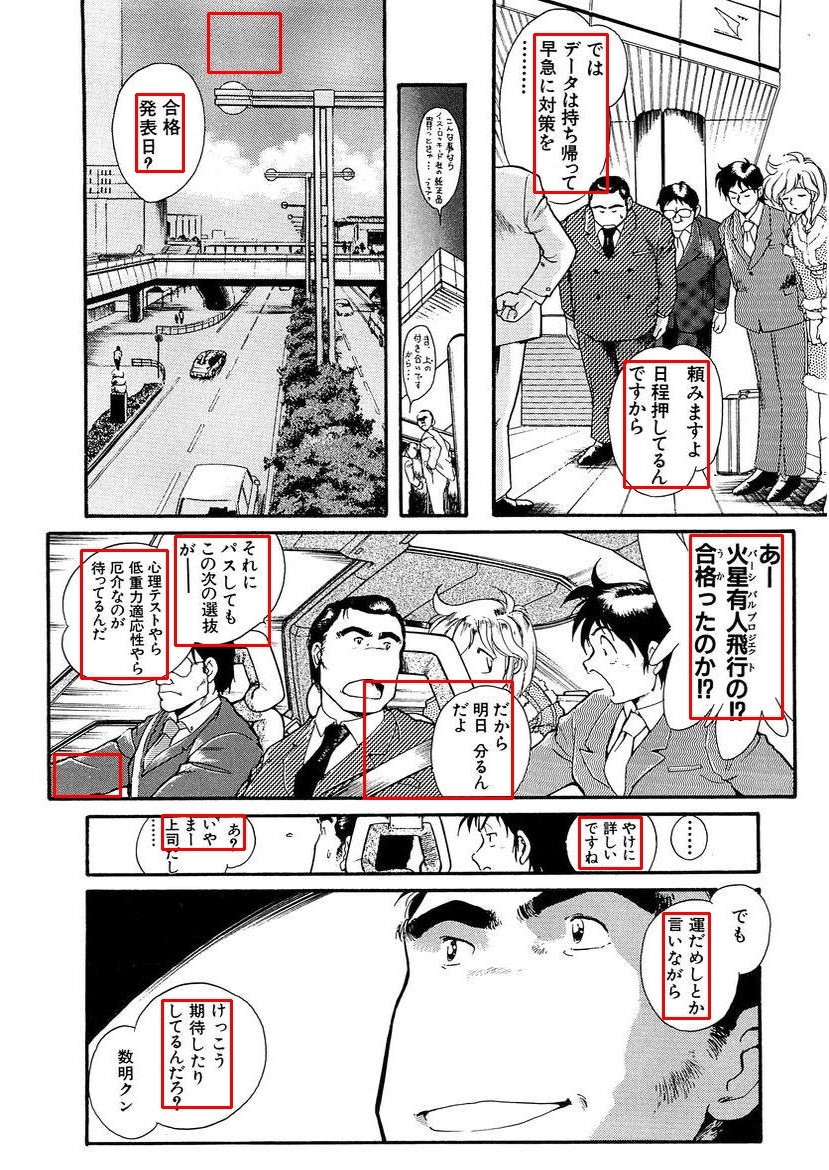
\includegraphics[width=0.45\textwidth]{images/result4.jpg}  
    }
    \caption{ตัวอย่างขอบเขตข้อความที่วิธีการของเราตรวจพบ (ก--ข) Love Hina \copyright Ken Akamatsu และ (ค--ง) Eva Lady \copyright Miyone Shi}
    \label{Fig:ExampleResult}
\end{figure}

เป็นที่น่าสนใจอย่างมากที่วิธีการของเราสามารถทำงานได้ดีกว่าเทคนิค Deep Learning ทั้งสองวิธี สมมติฐานแรกคือ BG+ImN นั้นใช้ ImageNet Classification Model~\cite{Krizhevsky} ซึ่งถูกเทรนบนภาพถ่ายของวัตถุจริง อย่างไรก็ดีภาพวาดมังงะของวัตถุต่าง ๆ นั้นมีความแตกต่างจากภาพวัตถุจริงอย่างชัดเจนซึ่ง ณ จุดนี้ทำให้วิธีการนี้ไม่สามารถทำงานได้เต็มประสิทธิภาพ อีกวิธีการที่ใช้ Deep Learning คือ BG+I2V ถึงแม้ว่าวิธีการนี้จะได้รับ Precision สูงที่สุดในการทดลองของเราแต่คะแนน Recal นั้นต่ำกว่าทั้ง BG+ImN และวิธีการของเรา วิธีการนี้ใช้โมเดล Illustration2Vec~\cite{Saito:2015:ISV:2820903.2820907} เป็นโมเดลสำหรับคัดแยกข้อความจากวัตถุอื่น ๆ ที่ปรากฎในภาพมังงะ ส่วนของโมเดลนั้นถูกเทรนบนภาพวาด Anime (ภาพการ์ตูนแบบญี่ปุ่น) และภาพมังงะจากหลากหลายแหล่งอันประกอบไปด้วย Danbooru และ Safebooru ซึ่งมีลักษณะงานคล้ายกับข้อมูลที่เราใช้ทดสอบในวิธีการของเรา แต่โมเดลนี้ถูกออกแบบมาเพื่อการทำนายป้ายกำกับ (Tag Prediction) และค้นหาภาพที่คล้ายคลึงกัน ดังนั้นการเลือกใช้วิธีการที่ไม่ต้องลักษณะงานโดยตรงในลักษณะนี้จึงอาจเป็นเหตุผลว่าทำไมโมเดลนี้จึงไมมีประสิทธิภาพเท่าที่ควรในการทดลองนี้

    \chapter{สรุปผล}
\label{chapter:conclusion}

บทที่ห้า

    \clearpage
    \addcontentsline{toc}{chapter}{บรรณานุกรม}
    \bibliographystyle{IEEEtran}
    \bibliography{reference}

    \startappendix
    \chapter{การใช้ชีวิตในประเทศญี่ปุ่น}

สำหรับการฝึกงานร่วมกับมหาวิทยาลัยฮอกไกโดในประเทศญี่ปุ่น ได้ทำการฝึกงานรวมกันเป็นระยะสี่เดือนกับอีกสิบวัน โดยได้เข้ามาทำงานในห้องทดลอง Intelligent Information System ภายใต้การดูแลของอาจารย์ประจำห้องทดลอง \Exami \ และในช่วงเวลาฝึกงานนี้ยังได้รับความช่วยเหลือจากสมาชิกภายในห้องทดลองอีกท่าน Jiang Ye นักศึกษาปริญญาเอก ปี 2 จากประเทศจีน ได้ให้ความช่วยเหลือและการดูแลในเรื่องการดำเนินการเอกสารที่จำเป็นต่าง ๆ เช่น เอกสารการย้ายเข้ามาพำนักในประเทศญี่ปุ่นและการย้ายออกจากประเทศญี่ปุ่น นอกจากนี้ยังได้รับความช่วยเหลือในเรื่องความเป็นอยู่และสิ่งของทั่วไปในการใช้ชีวิตจากทั้งกลุ่มนักศึกษาชาวไทยและชาวต่างชาติซึ่งล้วนศึกษาอยู่ที่มหาวิทยาลัยฮอกไกโด

การใช้ชีวิตในต่างแดน เช่น ประเทศญี่ปุ่นนั้นมีอุปสรรคหลายอย่าง ปัญหาประการหนึ่งที่ประสบบ่อยครั้งที่สุด คือ เรื่องการสื่อสารภาษาญี่ปุ่น อย่างที่ทราบกันดีว่าชาวญี่ปุ่นส่วนใหญ่ไม่สามารถสนทนาภาษาอังกฤษได้ ดังนั้นจึงมีความจำเป็นต้องเรียนรู้ภาษาญี่ปุ่นพื้นฐานเพื่อใช้ในการดำเนินชีวิตประจำวัน รวมถึงสมาชิกภายในห้องทดลองที่ส่วนใหญ่ไม่สามารถสื่อสารด้วยภาษาอังกฤษเช่นกัน สมาชิกภายในห้องทดลองส่วนมากจะสามารถสื่อสารได้เพียงประโยคพื้นฐาน ไม่สามารถสนทนาเป็นบทสนทนาที่ยาวหรือเป็นการเล่าเรื่องได้ แต่อย่างไรก็ดีพวกเขาสามารถอ่านและเขียนภาษาอังกฤษได้ค่อนข้างดี ดังนั้นเมื่อมีปัญหาในการพูดคุยจึงใช้การเขียนหรือพิมพ์ทดแทน อย่างไรก็ดีภายในห้องทดลองก็มีสมาชิกชาวญี่ปุ่นบางคนที่มีความสามารถภาษาอังกฤษในขั้นดีมาก อย่างเช่นนักศึกษาปริญญาโทชาวญี่ปุ่นท่านหนึ่งที่เคยได้ฝึกงานในนิวซีแลนด์และฟิลิปปินส์มาก่อนหน้านี้ทำให้สามารถสื่อสารภาษาอังกฤษได้เป็นอย่างดี

นอกจากตัวผมที่เป็นนักศึกษาฝึกงานจากไทย ภายในห้องทดลองที่ผมฝึกงานก็ยังมีนักศึกษาต่างชาติอีกสองคน คนแรกอย่างที่กล่าวไปในตอนต้น คือ นักศึกษาปริญญาเอกจากประเทศจีน และคนที่สองคือนักศึกษาปริญญาโทจากบราซิล สำหรับชาวจีนนั้นใช้ภาษาญี่ปุ่นเป็นภาษาหลักและสามารถสื่อสารกับคนญี่ปุ่นในห้องทดลองได้อย่างราบรื่น และยังพูดภาษาอังกฤษได้ดีอีกด้วย

\section{ที่อยู่อาศัย}

หอพักที่ใช้อาศัยตลอดโครงการฝึกงานนี้ถูกจัดหาให้โดยทางมหาวิทยาลัยฮอกไกโด หอพักมีชื่อว่า \textit{International House Kita 8 East} เป็นหอชายล้วนจัดให้สำหรับนักศึกษาชาวต่างชาติเท่านั้น โดยภายในห้องจะมีเพียงตู้, เตียง, โต๊ะ, โคมไฟ, ไฟเพดาน, ตู้เย็น, ฮีทเตอร์, และถังขยะ อย่างที่แสดงในภาพ~\ref{Fig:dorm:1} และ~\ref{Fig:dorm:2} สำหรับห้องน้ำ และห้องซักรีดต้องใช้ของส่วนกลางเท่านั้น โดยจะจัดแยกในแต่ละชั้นสำหรับให้ผู้อยู่อาศัยใช้ร่วมกัน

สำหรับห้องครัวและห้องรับประทานอาหารมีจัดเตรียมให้ที่ชั้นแรกของหอพักโดยต้องใช้ร่วมกันทั้งหอพัก เตาแก๊สและอ่างล้างจานถูกติดตั้งไว้เรียบร้อยสามารถใช้งานได้ในทันที สำหรับของใช้ส่วนตัวรวมถึงเครื่องครัวผู้อยู่อาศัยต้องหาซื้อด้วยตนเอง ในกรณีของผมมีความจำเป็นซื้อแค่ชุดจานชามช้อนซ้อมและแก้ว สำหรับอุปกรณ์ทำอาหารได้รับมาจากนักศึกษาชาวจีนที่กำลังจะกลับประเทศจีน ภาพห้องครัวแสดงในภาพ~\ref{Fig:dorm:3} และ~\ref{Fig:dorm:4}

\begin{figure}[!h]
    \centering
    \subfigure[ห้องนอน]{
        \label{Fig:dorm:1}
        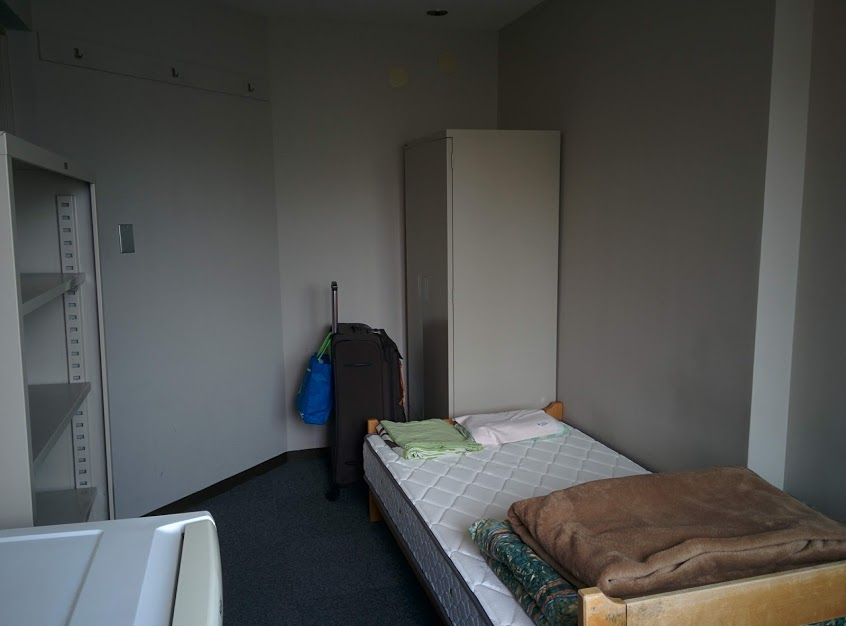
\includegraphics[width=0.45\linewidth]{dorm1}
    }
    \subfigure[ห้องนอน]{
        \label{Fig:dorm:2}
        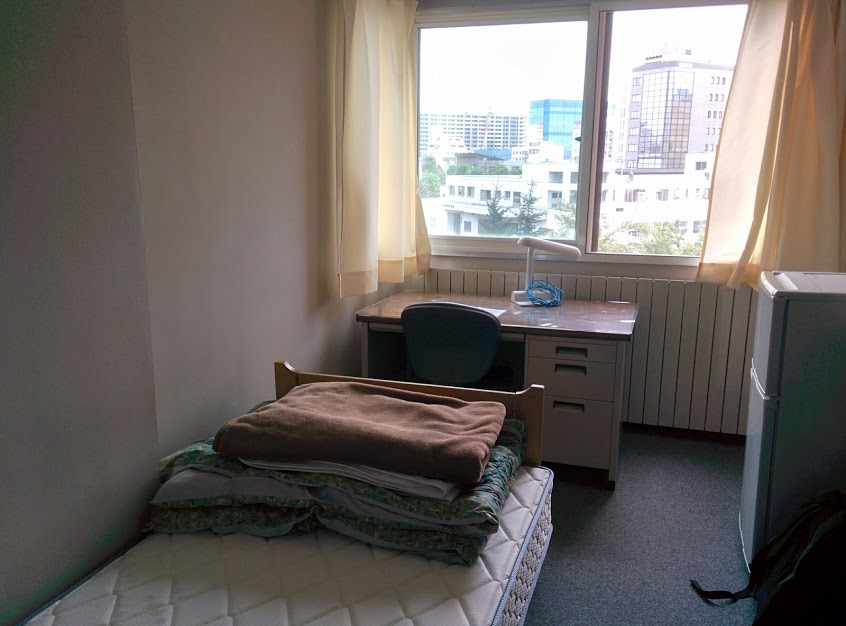
\includegraphics[width=0.45\linewidth]{dorm2}
    }
    \subfigure[ห้องอาหาร]{
        \label{Fig:dorm:3}
        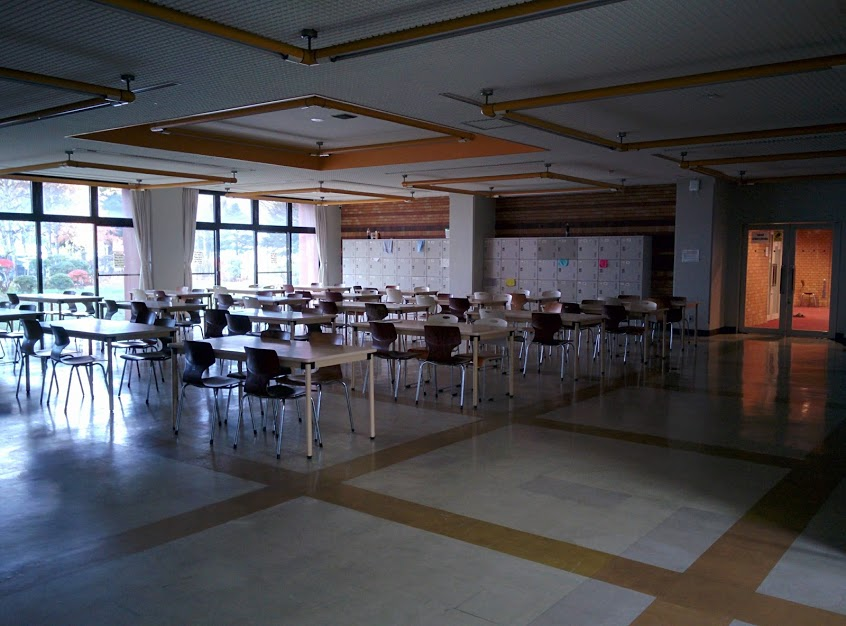
\includegraphics[width=0.45\linewidth]{dorm4}
    }
    \subfigure[ห้องครัว]{
        \label{Fig:dorm:4}
        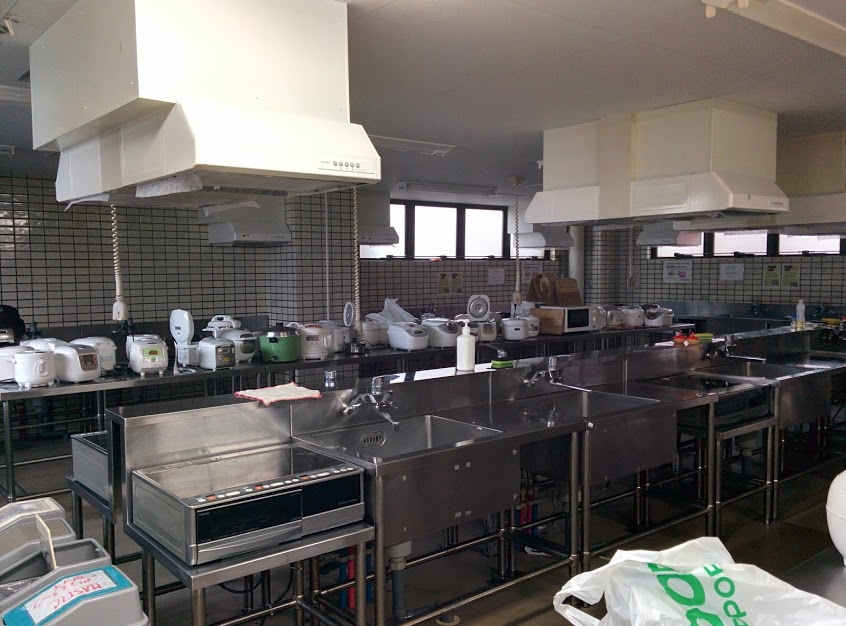
\includegraphics[width=0.45\linewidth]{dorm3}
    }
    \caption{ภาพหอพัก International House Kita 8 East}
    \label{Fig:dorm}
\end{figure}

\chapter{กิจกรรมระหว่างฝึกงาน}

นอกจากการมาทำโปรเจคแล้วนั้น ระหว่างสี่เดือนนี้ผมยังได้ร่วมกิจกรรมด้านวิชาการต่าง ๆ ดังเช่น การประชุมห้องทดลองรายสัปดาห์ และ การร่วมนำเสนอผลงานระหว่างห้องทดลอง เป็นต้น โดยรายละเอียดจะกล่าวต่อจากนี้

\section{Mirai Symposium}

กิจกรรมนี้จัดขึ้นที่เรียวกังหรือรีสอร์ทแบบญี่ปุ่น ซึ่งมีออนเซ็นหรือบ่อน้ำพุร้อนให้ได้แช่อีกด้วย ค่าใช้จ่ายทั้งหมดทางห้องทดลองออกให้ทั้งหมด ภายในงานจะมีกิจกรรมหลักคือการให้นักศึกษาทุกคนของห้องทดลองต่าง ๆ ที่มาร่วมงานนำผลงานตนเองมานำเสนอด้วยโปสเตอร์ในห้องประชุม หมุนเวียนไปเป็นช่วงเวลาคนละ 30 นาที หากสนใจงานของใครก็สามารถเดินไปสอบถามได้ อย่างที่เห็นในภาพ~\ref{Fig:mirai:1} การนำเสนอไม่ได้จำกัดว่างานต้องเป็นผลงานที่เสร็จสิ้นแล้ว อาจเป็นความก้าวหน้าของงานที่พัฒนาอยู่ได้เช่นเดียวกัน สำหรับครั้งนี้มีห้องทดลองร่วมงานสามห้องทดลอง สำหรับนักศึกษาต่างชาติจะมีนักศึกษาท่านอื่นเข้ามาสอบถามเพียงเล็กน้อยเนื่องจากต้องสื่อสารด้วยภาษาอังกฤษและนักศึกษาญี่ปุ่นส่วนใหญ่ไม่สามารถพูดอังกฤษได้ สำหรับงานวิจัยที่ผมพัฒนาก็ได้นำไปนำเสนอในงานนี้ด้วยเช่นเดียวกัน

เมื่อช่วงนำเสนอเสร็จสิ้น ทุกคนจะได้พักผ่อนตามอัธยาศัยโดยส่วนใหญ่จะเลือกไปแช่บ่อน้ำพุร้อนกัน สำหรับบ่อน้ำพุร้อนก็มีทั้งภายนอกและภายในอาคาร จากนั้นเป็นมื้อเย็นซึ่งเป็นอาหารชุดญี่ปุ่น~\ref{Fig:mirai:2}

\begin{figure}[!h]
    \centering
    \subfigure[บรรยากาศระหว่างการนำเสนอผลงานด้วยโปสเตอร์]{
        \label{Fig:mirai:1}
        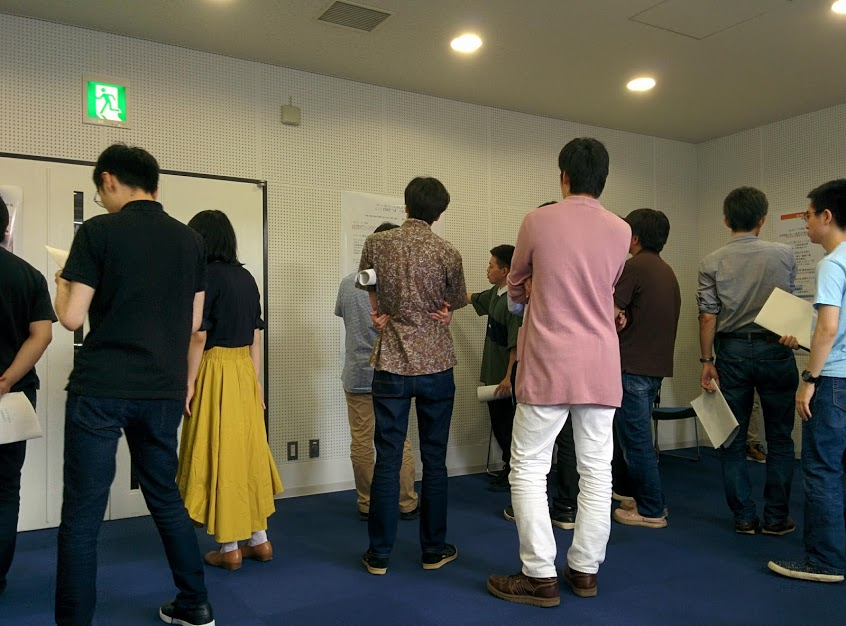
\includegraphics[width=0.8\linewidth]{mirai1}
    }
    \subfigure[ชุดอาหารจัดเลี้ยงมื้อเย็น]{
        \label{Fig:mirai:2}
        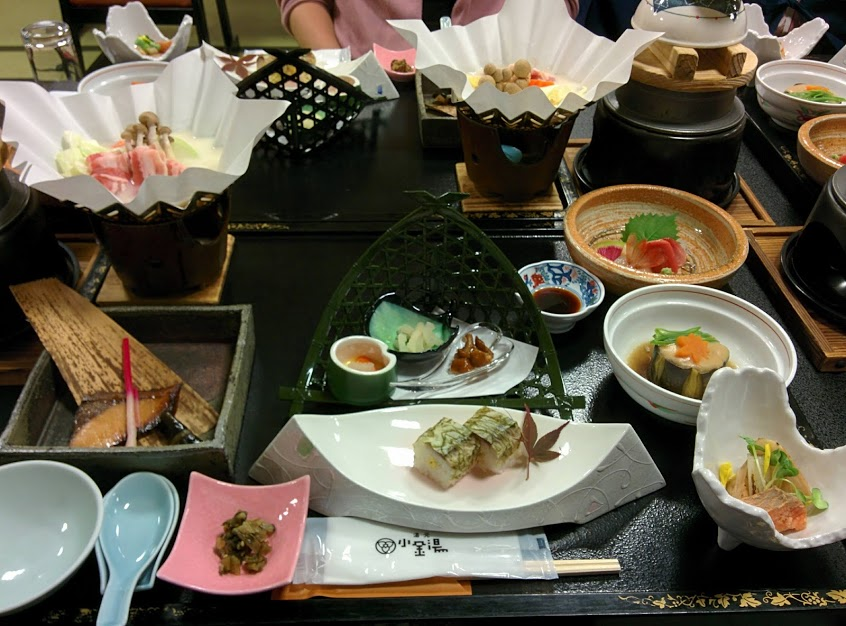
\includegraphics[width=0.45\linewidth]{mirai2}
    }
    \subfigure[ห้องอาหารจัดเลี้ยง]{
        \label{Fig:mirai:3}
        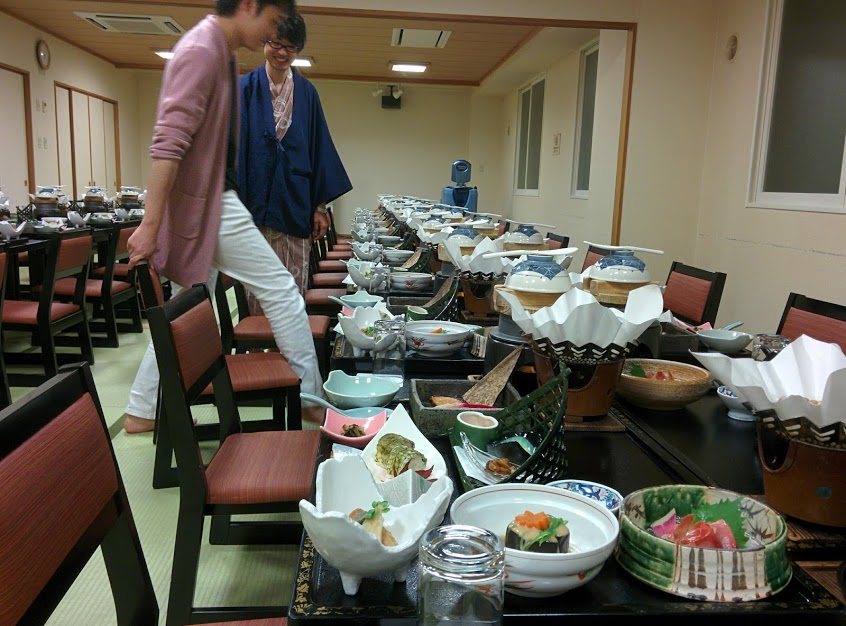
\includegraphics[width=0.45\linewidth]{mirai3}
    }
    \caption{ภาพกิจกรรมในงาน Mirai Symposium}
    \label{Fig:mirai}
\end{figure}

สำหรับวันที่สองก็มีกิจกรรมสร้างสรรค์ เป็นกิจกรรมที่ให้แยกกลุ่มกันและแก้โจทย์ปัญหาโดยให้แก้ภายในเวลาที่กำหนด ตัวอย่างคำถามเช่น \textit{มีเหรียญอยู่ร้อยเหรียญมีทั้งที่หงายหน้าก้อยและหัวอย่างละครึ่ง ต้องการแบ่งกลุ่มเหรียญสองกลุ่มโดยที่แต่ละกลุ่มมีจำนวนหน้าเหรียญและก้อยเท่า ๆ กัน โดยที่ผู้แบ่งมองไม่เห็นเหรียญจะทำได้อย่างไร} เป็นต้น เมื่อเสร็จกิจกรรมสร้างสรรค์ก็ถือเป็นการจบกิจกรรม Mirai Symposium แต่เพียงเท่านี้และเดินทางกลับมหาวิทยาลัย

\section{Lab Meeting}

สำหรับท้องทดลองที่ได้เข้ามาฝึกงานนั้นมีกิจกรรม Lab Meeting ทุกวันพุธ คือ กิจกรรมที่ให้สมาชิกภายในห้องทดลองร่วมกันนำงานวิจัยต่าง ๆ ที่ได้อ่านมานำเสนอต่อสมาชิกท่านอื่น ๆ ภายในห้องทดลอง โดยแต่ละสมาชิกจะถูกกำหนดวันเพื่อให้แต่ละคนที่ถูกกำหนดในวันนั้นนำ Conference Paper หรือ Journal ที่ถูกตีพิมพ์ในงานประชุมวิชาการชื่อดังของโลกมาร่วมกันนำเสนอแบบสรุปพร้อมสไลด์ กิจกรรมนี้ไม่มีคะแนนหรือรางวัลใด ๆ แต่เป็นการแลกเปลี่ยนความรู้ที่เกี่ยวข้องกับงานของตนเองที่ทำอยู่ 

สำหรับผมได้มีโอกาสนำเสนองานวิจัยที่ถูกตีพิมพ์ใน Journal เรื่อง \textit{Text-aware balloon extraction from manga} โดยหลังจากนำเสนอเสร็จสิ้นก็ได้รับคำถามและความคิดเห็นจากสมาชิกและอาจารย์ของห้องทดลองอย่างหลากหลาย ซึ่งถือเป็นโอกาสที่ดีในการเรียนรู้มุมมองและความคิดเห็นที่แปลกใหม่ต่องานของเรา

\section{กิจกรรมอื่น ๆ}

นอกจากกิจกรรมเชิงวิชาการแล้ว ผมยังได้ร่วมในกิจกรรมสังสรรค์อื่น ๆ เช่น งานเลี้ยงตามโอกาสต่าง ๆ โดยผมได้ร่วมงานเลี้ยงต้อนรับตัวผม ซึ่งจัดในช่วงเดือนตุลาคมที่ผ่านมา สาเหตุที่จัดช้าจากเดือนที่เข้าฝึกงานวันแรกไปหลายเดือนเนื่องจากกำหนดการในตอนแรกนั้นคือหนึ่งเดือนหลังจากผมมาอยู่ที่ประเทศญี่ปุ่น แต่ในช่วงกำหนดการเกิดเหตุการณ์แผ่นดินไหวใหญ่บนเกาะฮอกไกโดทำให้ต้องเลื่อนกำหนดการออกไป โดยงานเลี้ยงนี้จัดที่ร้านเนื้อย่างเจงกิสข่าน เป็นเนื้อแกะย่างบนเตาเหล็กลักษณะคล้ายหมูกระทะในประเทศไทยแตกต่างกันเพียงเน้นไปที่เนื้อแกะเป็นหลัก ภาพกิจกรรมแสดงในภาพ~\ref{Fig:welcome-party}

\begin{figure}[!h]
    \centering
    \subfigure[สมาชิกในห้องทดลองระหว่างกินเลี้ยง]{
        \label{Fig:welcome-party:1}
        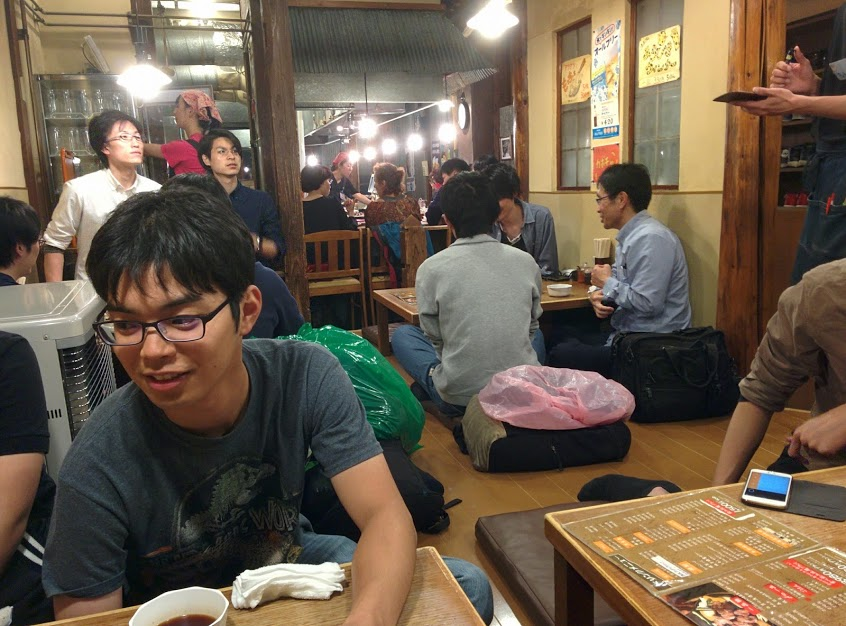
\includegraphics[width=0.8\linewidth]{welcome-party-1}
    }
    \subfigure[โต๊ะอาหารในร้านอาหารเจงกิสข่าน]{
        \label{Fig:welcome-party:2}
        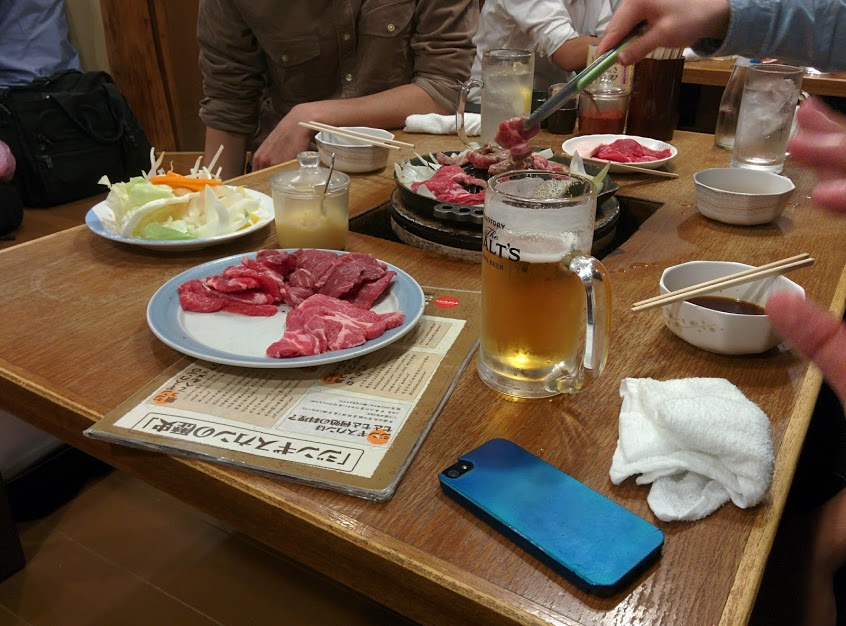
\includegraphics[width=0.45\linewidth]{welcome-party-2}
    }
    \subfigure[กระทะร้อนเจงกิสข่าน]{
        \label{Fig:welcome-party:3}
        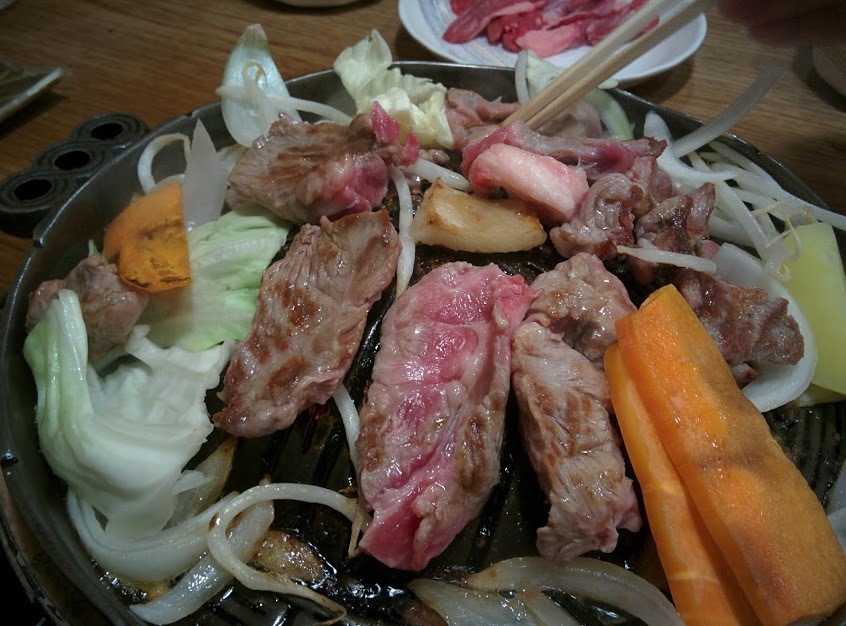
\includegraphics[width=0.45\linewidth]{welcome-party-3}
    }
    \caption{ภาพระหว่างงานเลี้ยงต้อนรับ}
    \label{Fig:welcome-party}
\end{figure}

นอกจากงานเลี้ยงต้อนรับแล้วยังมีงานเลี้ยงต้อนรับนักศึกษาปีสามที่เข้าเป็นสมาชิกใหม่ในห้องทดลองนี้อีกด้วย ซึ่งงานนี้จัดรวมเป็นงานเลี้ยงอำลาตัวผมพร้อม ๆ กันเนื่องจากจัดใกล้วันสิ้นสุดการฝึกงาน งานเลี้ยงจัดในห้องทดลองพร้อมด้วยอาหารหลากหลายชนิด งานไม่มีกิจกรรมอะไรมากมายเป็นเพียงการกินเลี้ยงเพื่อทำความรู้จักกับสมาชิกใหม่ของห้องทดลองและนั่งเล่นเกมด้วยกินตามที่แสดงในภาพ~\ref{Fig:farewell-party}

\begin{figure}[!h]
    \centering
    \subfigure[อาหารต่าง ๆ ในงานเลี้ยง]{
        \label{Fig:farewell:1}
        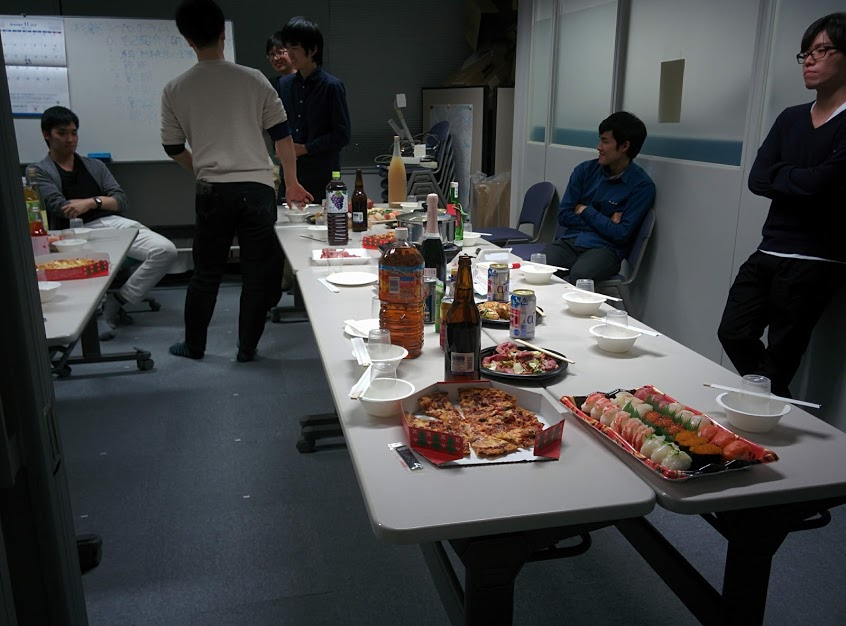
\includegraphics[width=0.8\linewidth]{farewell-party-1}
    }
    \subfigure[สมาชิกในห้องทดลองระหว่างเล่นเกมในงานเลี้ยง]{
        \label{Fig:farewell:2}
        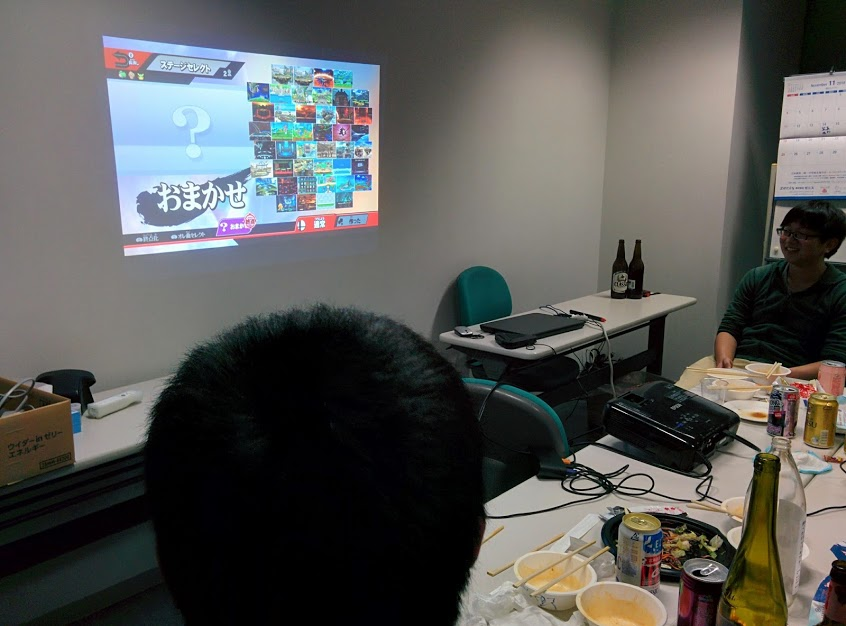
\includegraphics[width=0.8\linewidth]{farewell-party-2}
    }
    \caption{งานเลี้ยงอำลาและต้อนรับนักศึกษาปีสาม}
    \label{Fig:farewell-party}
\end{figure}

อธิบายเพิ่มเติมสำหรับงานเลี้ยงต้อนรับนักศึกษาปีสาม สำหรับห้องทดลองของคณะวิศวกรรมศาสตร์ที่ได้มาอยู่นี้จะมีการเปิดห้องทดลองให้นักศึกษาในคณะชั้นปีสามได้เข้าเยี่ยมชมห้องทดลองที่ตนเองสนใจก่อนจะเลือกเข้ามาเป็นสมาชิกในห้องทดลองที่เกี่ยวข้องกับงานที่สนใจจะทำ โดยงานที่สนใจจะทำจะกลายเป็นชิ้นงานจบการศึกษาคล้ายกับในมหาวิทยาลัยของไทย โดยในช่วงเวลานี้ของปีแต่ละห้องทดลองก็จะมีการโฆษณาห้องทดลองของตัวเองและเปิดโอกาสให้เข้าเยี่ยมชมงานภายในห้องทดลองว่าทำวิจัยเรื่องอะไร อย่างเช่นภาพ~\ref{Fig:ads} ที่เป็นป้ายเชิญเข้าชมห้องทดลองด้านเสียงและมีการใช้ตัวละครจากการ์ตูนเรื่อง Kemono Friend ประกอบให้น่าสนใจและดึงดูดมากขึ้น

\begin{figure}
    \centering
    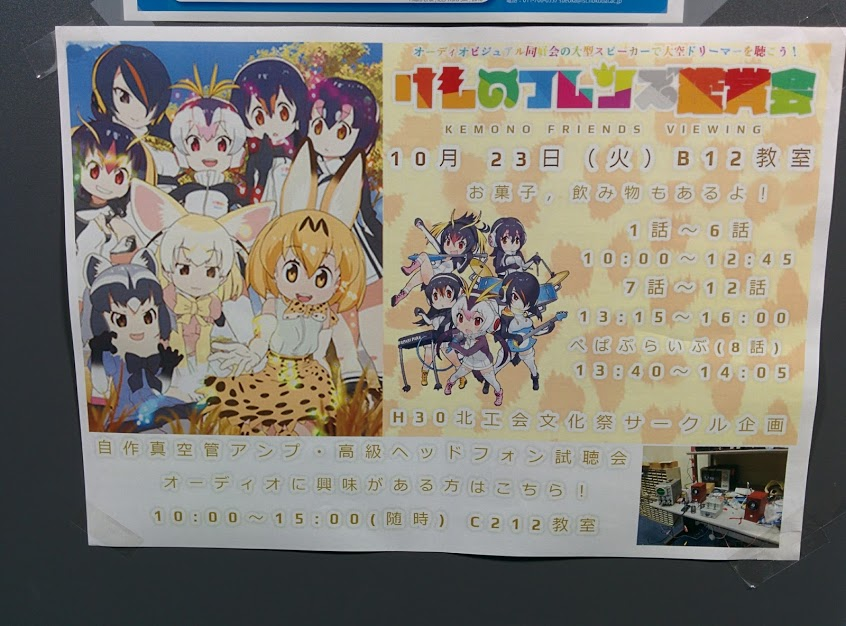
\includegraphics[width=0.8\linewidth]{ads}
    \caption{ป้ายเชิญชวนชมห้องทดลองโดยมีการใช้ตัวละครจากการ์ตูนประกอบให้น่าสนใจมากขึ้น}
    \label{Fig:ads}
\end{figure}

\clearpage 
\thispagestyle{empty}
\begin{center}
	\vspace*{\stretch{1}}
	\LARGE{\textbf{ภาคผนวก ค}}
	\vspace*{\stretch{1}}
\end{center}

\clearpage 
\thispagestyle{empty}
\begin{center}
    \vspace*{\stretch{1}}
    \LARGE{\textbf{ผลงานวิจัยที่ได้รับการตีพิมพ์}}
    \vspace*{\stretch{1}}
\end{center}

\addcontentsline{toc}{chapter}{ภาคผนวก\hspace{1ex}ค\hspace{2mm}ผลงานวิจัยที่ได้รับการตีพิมพ์}
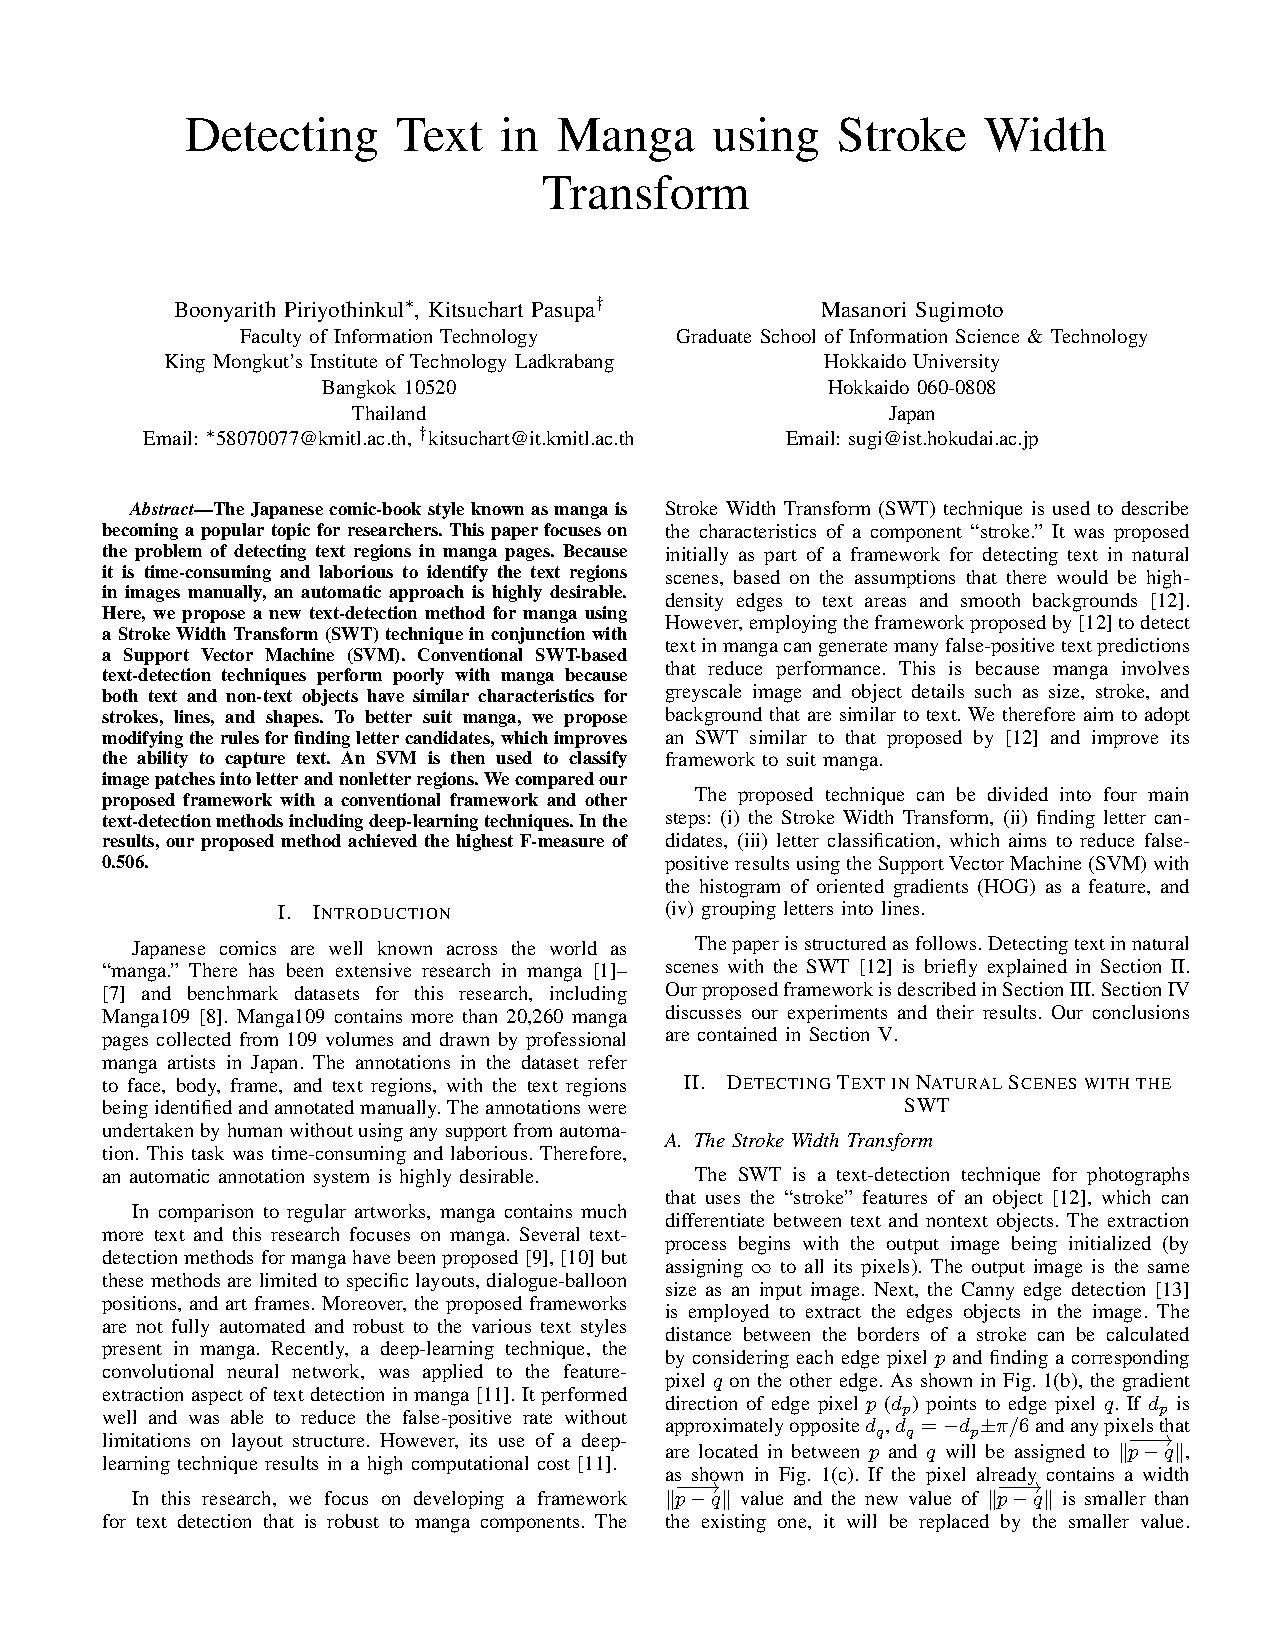
\includepdf[pages=-,pagecommand={}]{paper.pdf}

\end{document}
